\chapter{Hardware}
To carry out the commanded motion, the desired platform velocity vector is mapped into individual wheel angular velocities through an inverse Jacobian transformation:
% - Hardware layout of the testing ground, Show what we have this sem 
% - Compare the CAD Model and the IRL 
% - Exploded view of CAD Model and explain the layers
% - How we made the robot (Show the accuracy of the print with caliper)
    % - Camera Mount 
    % - Base iteration v1 v2
    % - Cutting of the shaft 
    % - Bearing?
    % - Bill of material
% - ..Maybe.. Talk about the robot kinematic
% - Currently implemented & exploring ESP32 with Embedded C

This chapter will be covering the work done, and the knowledge accumulated in the hardware section. Last semester no demonstration was done in hardware, all was done in simulation to focus on the communication which is the foundation of a decentralized robotics swarm system. This semester all the work done have been extended and implemented into hardware. 

%------------------------------------------------------------
\section{Hardware Layout}
The requirements for the hardware are the following:

\begin{enumerate}
    \item \textbf{Location}: Lab where a sterile arena can be implemented with minimal interruptions, Chulapat 14
    \item \textbf{Size}: 3-4 square meters of space, 2.1m x 1.4m
    \item \textbf{Floor}: Non-Refelective Floor to optimize for the computer vision system, White Paper floor
    \item \textbf{Barrier}: Barrier against a runaway robot, abandoned Metal Boxes
\end{enumerate}
In addition to the layout, a C-Stand supporting a Logitech C920 webcam for robot position validation and camera odometry. More information are provided in the Localization section




%------------------------------------------------------------
\section{Robot}
% - Compare the CAD Mod tl and the IRL 
In last semester midpoint point we have planned out the hardware contruction in CAD before developing in hardware, In Fig \ref{robot-cad}, is the what was model, the footprint of the robot is fairly small at 20cm \ref{robot-drawing} ilustrate the dimension of the each perspective of robot.

\begin{figure}
    \centering
    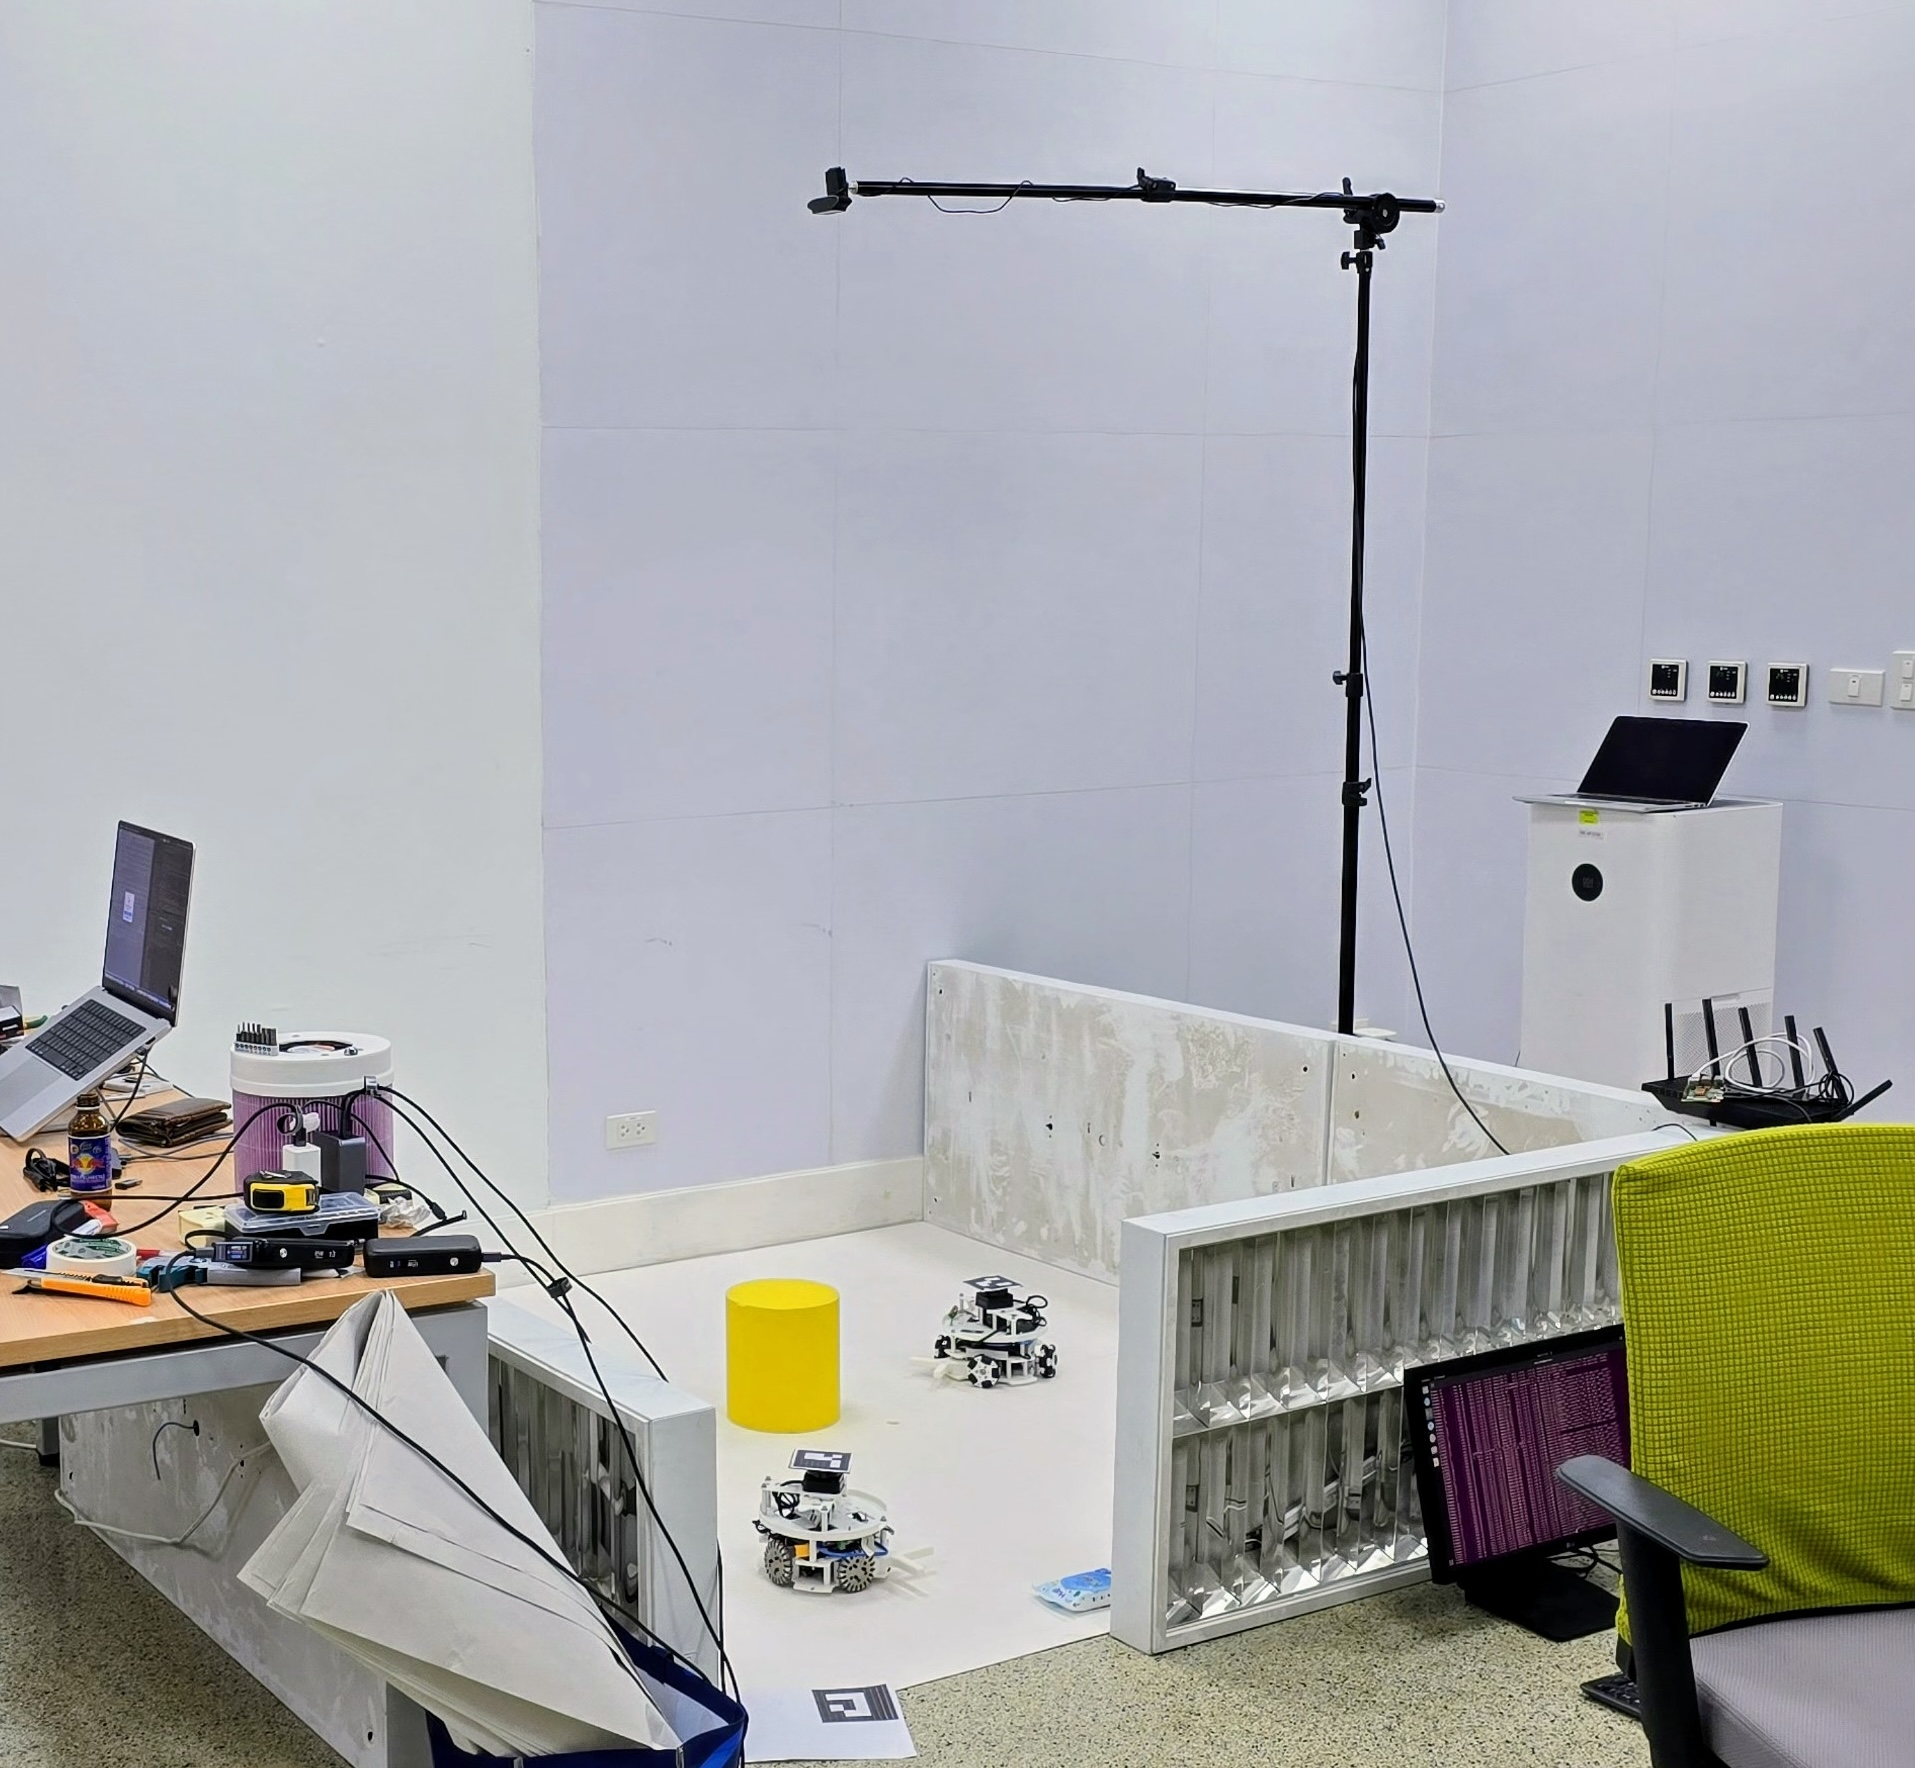
\includegraphics[width=0.65\linewidth]{assets/images/hardware/room-layout.jpg}
    \caption{Test Arena layout for the swarm project with a camera setup}
    \label{fig:have2robots}
\end{figure}

PLA+ frame is printed with a Bambu Lab P1S. PLA+ is chosen due to the ease of printing, eco-friendly, stiffness. Other material such as ABS and ASA or PETG, however, these release toxic fumes, flex more than PLA+. \ref{irl-robot} is the final forum of the robot. The rational behind using 3D printing as an alternative to 3D printing was due to the speed at which things can be prototyped. With modern printing like a Bambulab the accuracy are very good with tolerance of 0.2mm with good modeling design in mind with such as thermal expansion after printing. Resulting in ability to press fit the bearing all eight Bearing 626ZZ to the 3D printed bearing pillow holder. 

The vision aspect of the robot consist of the RPLiDAR S3 and a Logitech C920, Both of which require a custom 3D printed mount. 
The C920 require measurements using a vernier caliper as there's no publically avaliable CAD model, unlike the RPLiDAR S3. With no visiable mounting on the C920 the monitor stand was taken out and a 3D model of the enclosure is designed using the Snap Fit feature found in the Fusion 360(Learnt in Robotics Project IV), see \ref{cad-snap-fit-1} and \ref{cad-snap-fit-2}. 

\section{Robot Drive Train and kinematic}
The motors used are the Dynamixel 


\begin{figure}[!htb]
    % \centering
    \begin{minipage}{0.41\textwidth}
        % \centering
        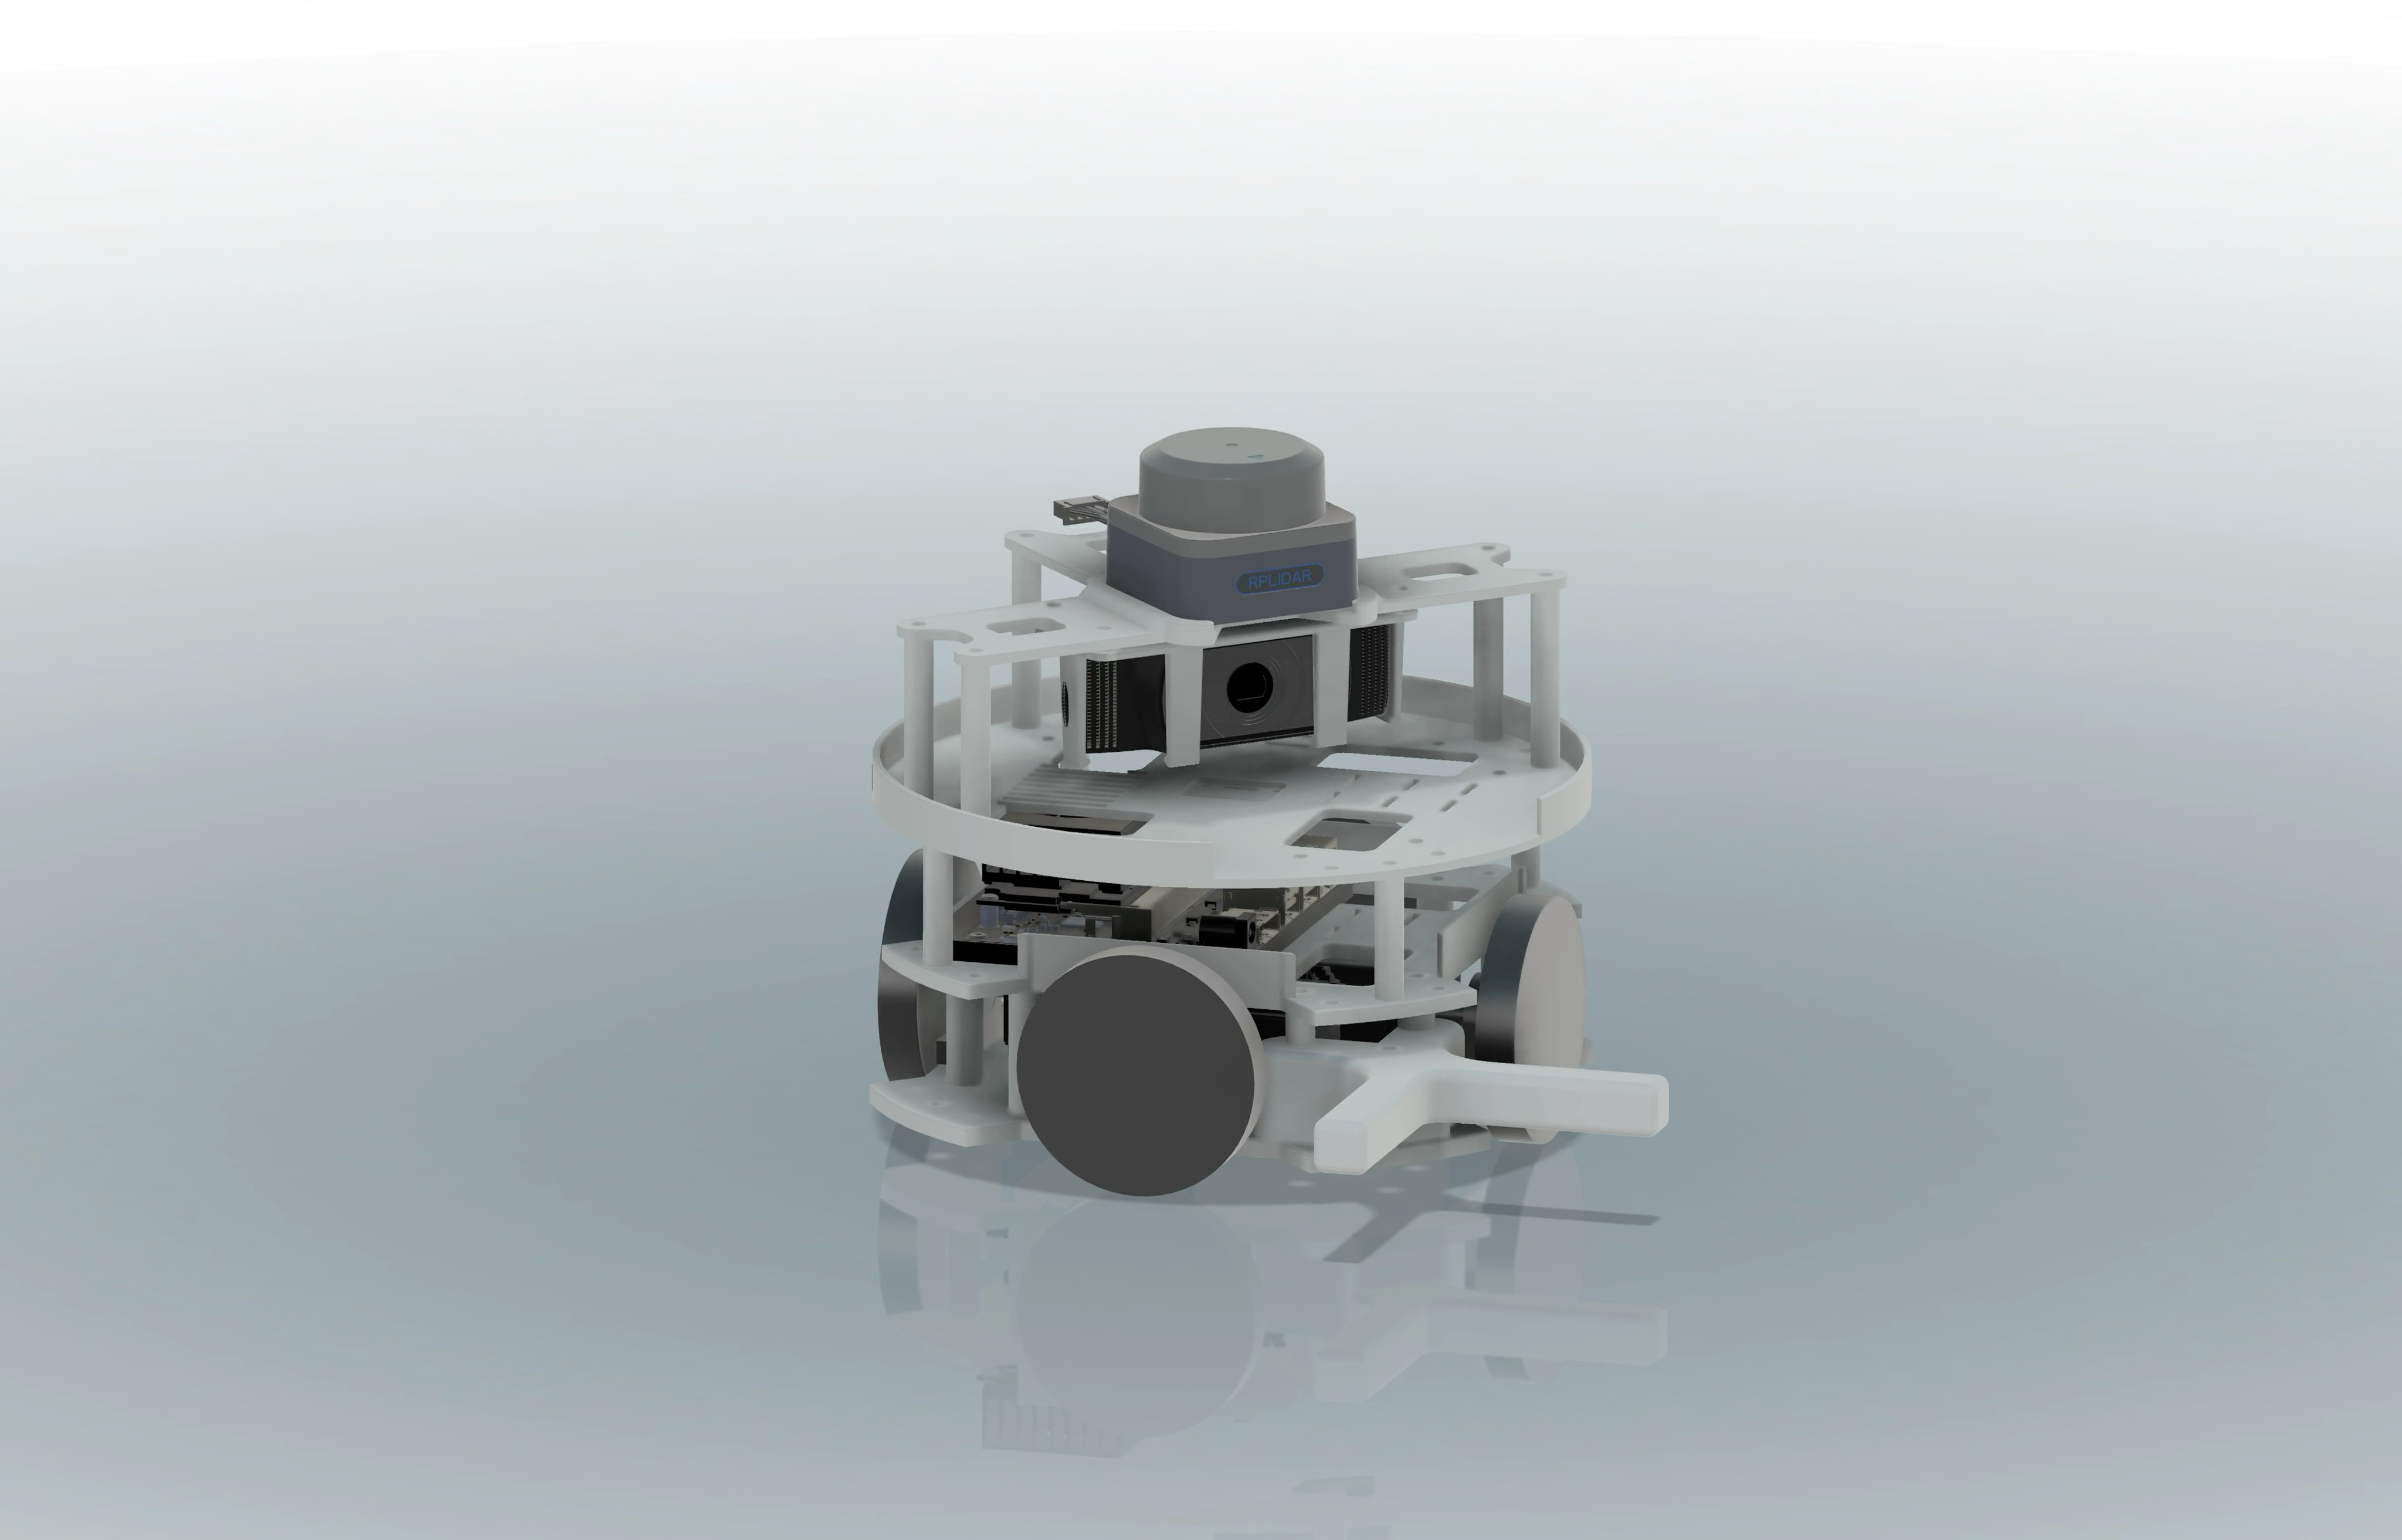
\includegraphics[height=5cm]{assets/images/hardware/robot-model.png}
        \caption{CAD Model of the designed robot named Jeff3}
        \label{fig:robot-cad}
    \end{minipage}
    \hspace{0.1\textwidth} % Add horizontal space here
    \begin{minipage}{0.41\textwidth}
        % \centering
        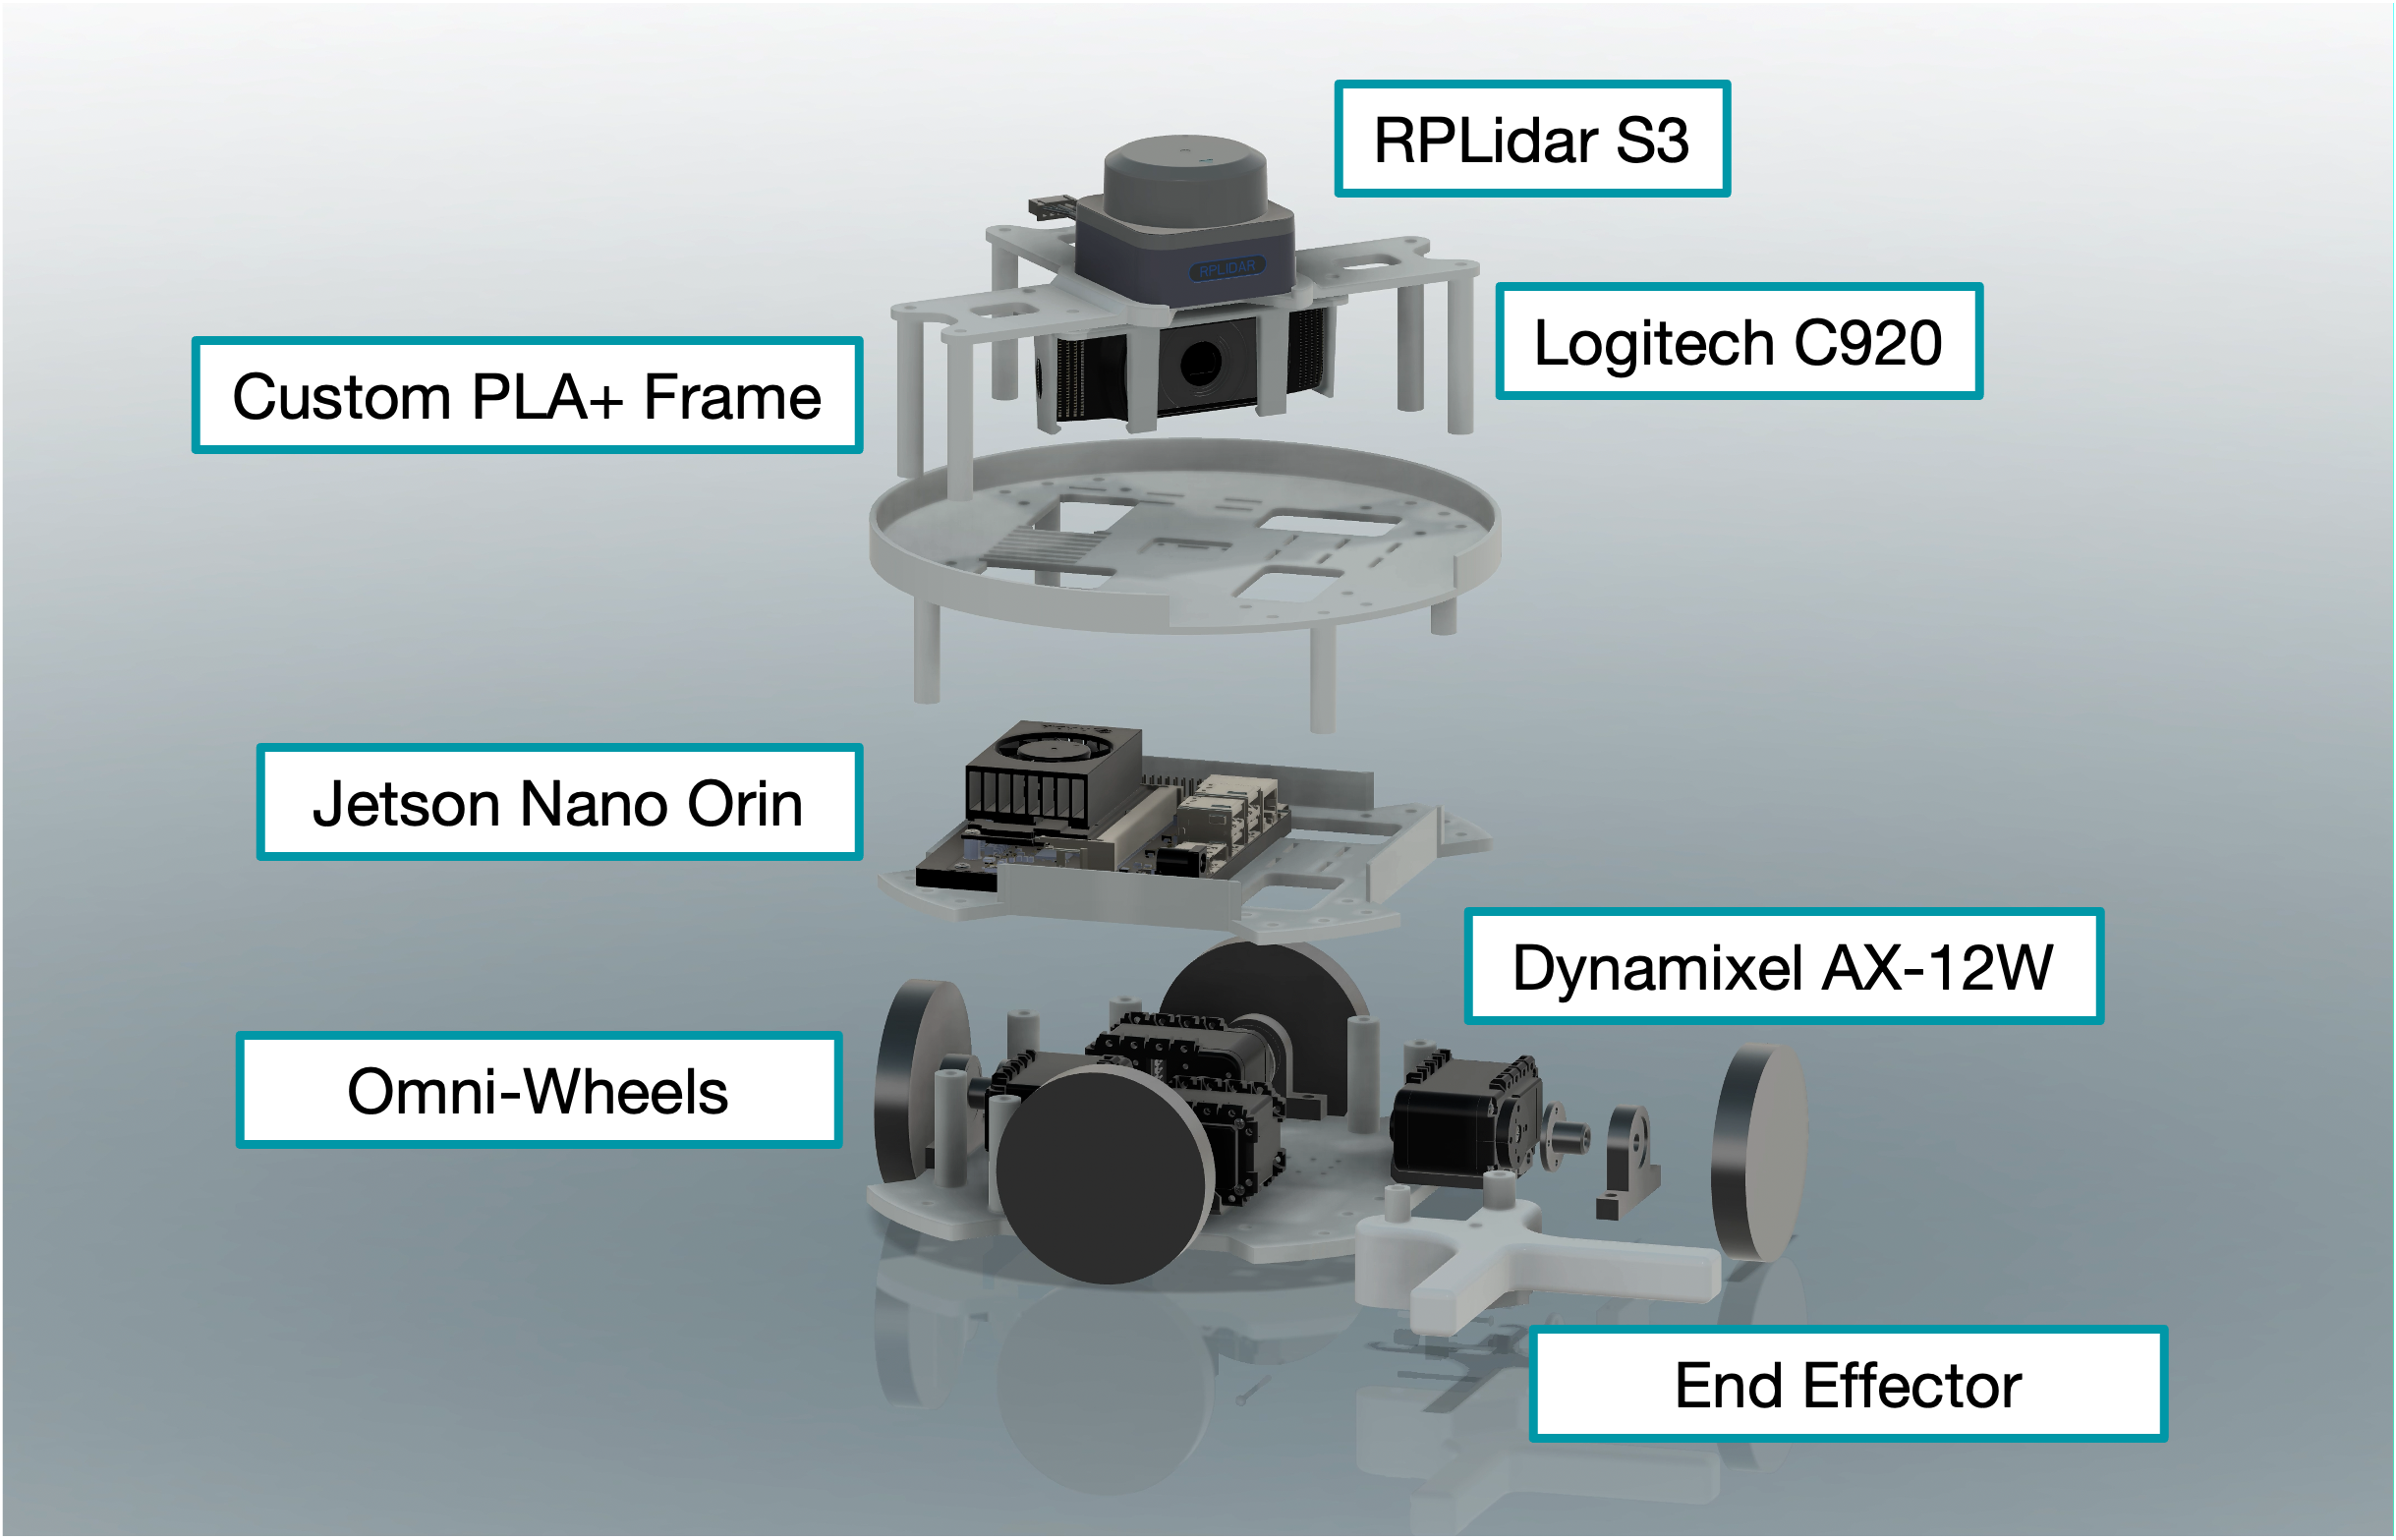
\includegraphics[height=5cm]{assets/images/hardware/robot-exploded-annotated.png}
        \caption{CAD Model of Robot Jeff3 annotated}
        \label{fig:robot-exploded}
    \end{minipage}
\end{figure}

\begin{figure}[!htb]
    % \centering
    \begin{minipage}{0.41\textwidth}
        % \centering
        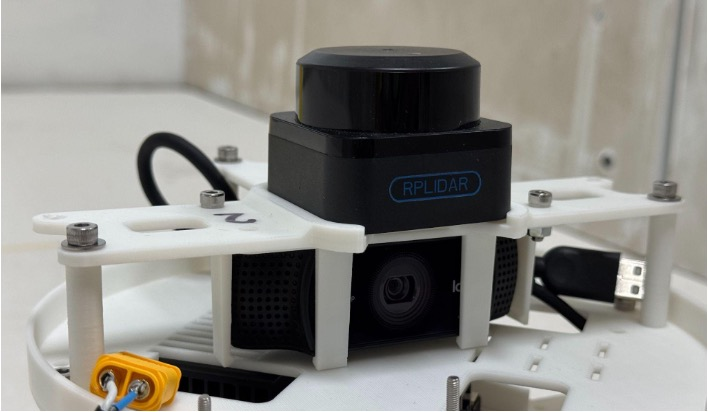
\includegraphics[height=5cm]{assets/images/hardware/irl-cameramount.jpg}
        \caption{}
        \label{fig:irl-snap-fit}
    \end{minipage}
    \hspace{0.1\textwidth} % Add horizontal space here
    % \begin{minipage}{0.41\textwidth}
    %     % \centering
    %     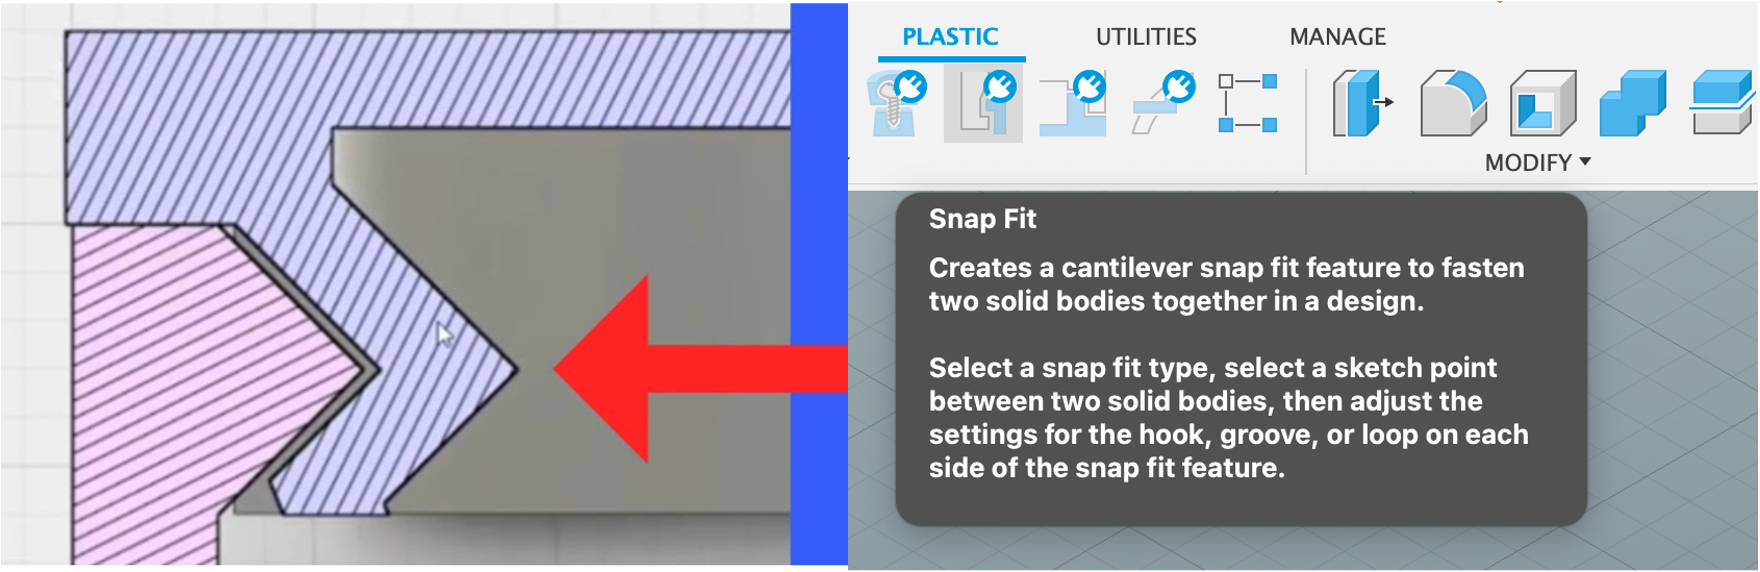
\includegraphics[height=5cm]{assets/images/hardware/cad-snapfit.png}
    %     \caption{}
    %     \label{fig:cad-snap-fit}
    % \end{minipage}
\end{figure}

\begin{figure}[!htb]
    % \centering
    \begin{minipage}{0.41\textwidth}
        % \centering
        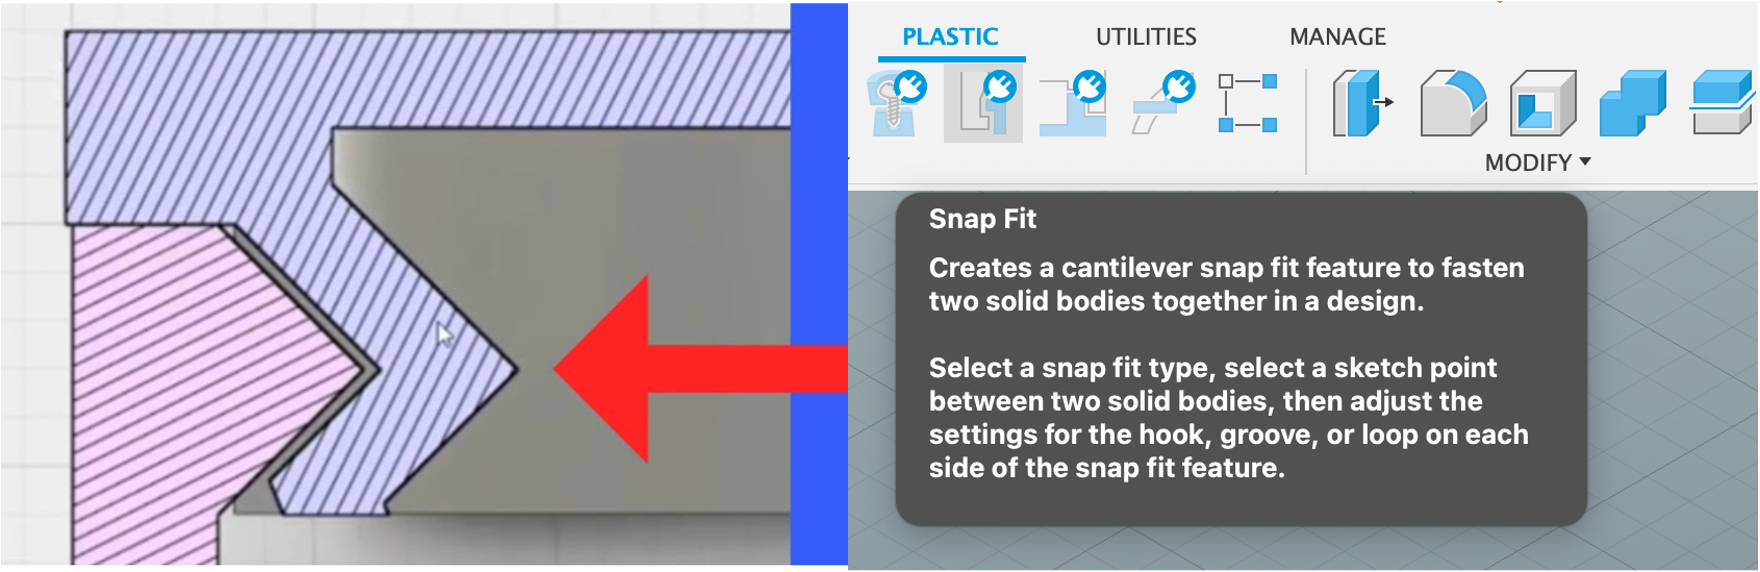
\includegraphics[height=5cm]{assets/images/hardware/cad-snapfit.png}
        \caption{}
        \label{fig:cad-snap-fit-1}
    \end{minipage}
    \hspace{0.1\textwidth} % Add horizontal space here
    \begin{minipage}{0.41\textwidth}
        % \centering
        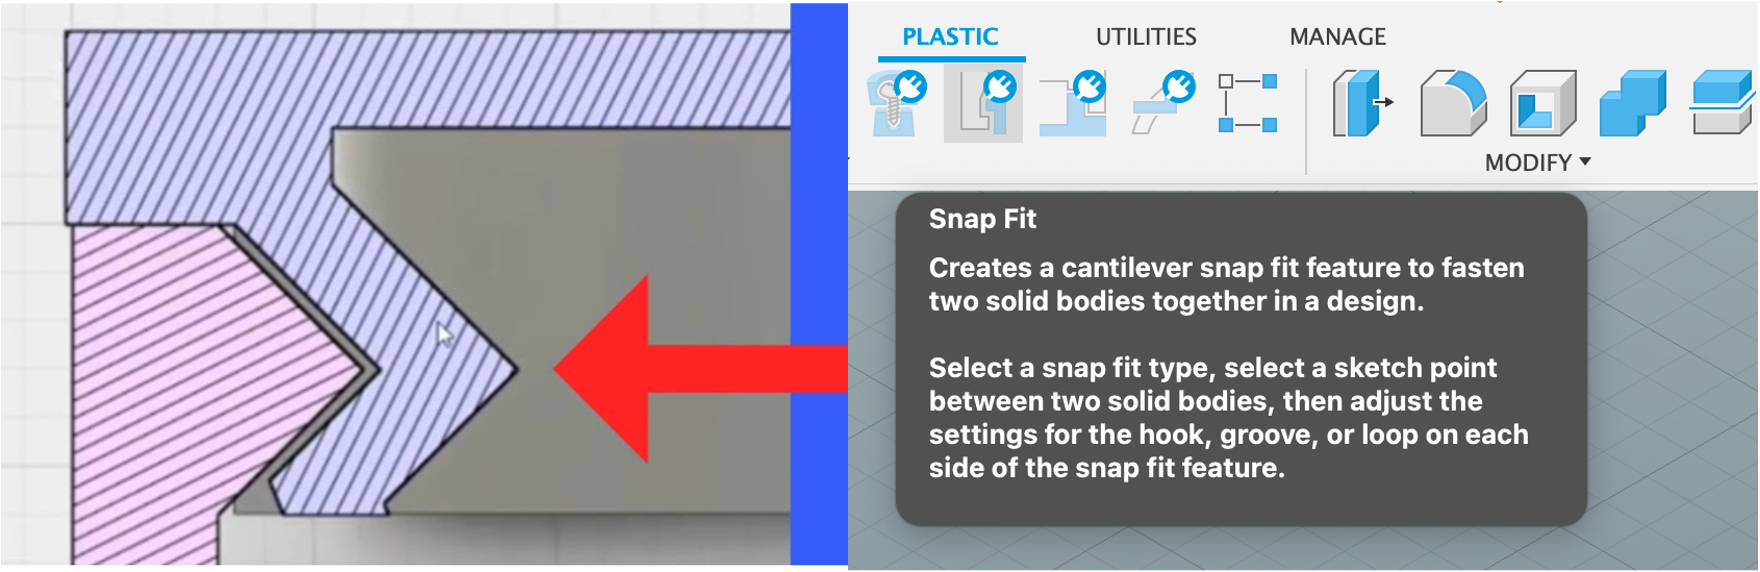
\includegraphics[height=5cm]{assets/images/hardware/cad-snapfit.png}
        \caption{}
        \label{fig:cad-snap-fit-2}
    \end{minipage}
\end{figure}

\begin{figure}[!htb]
    % \centering
    \begin{minipage}{0.41\textwidth}
        % \centering
        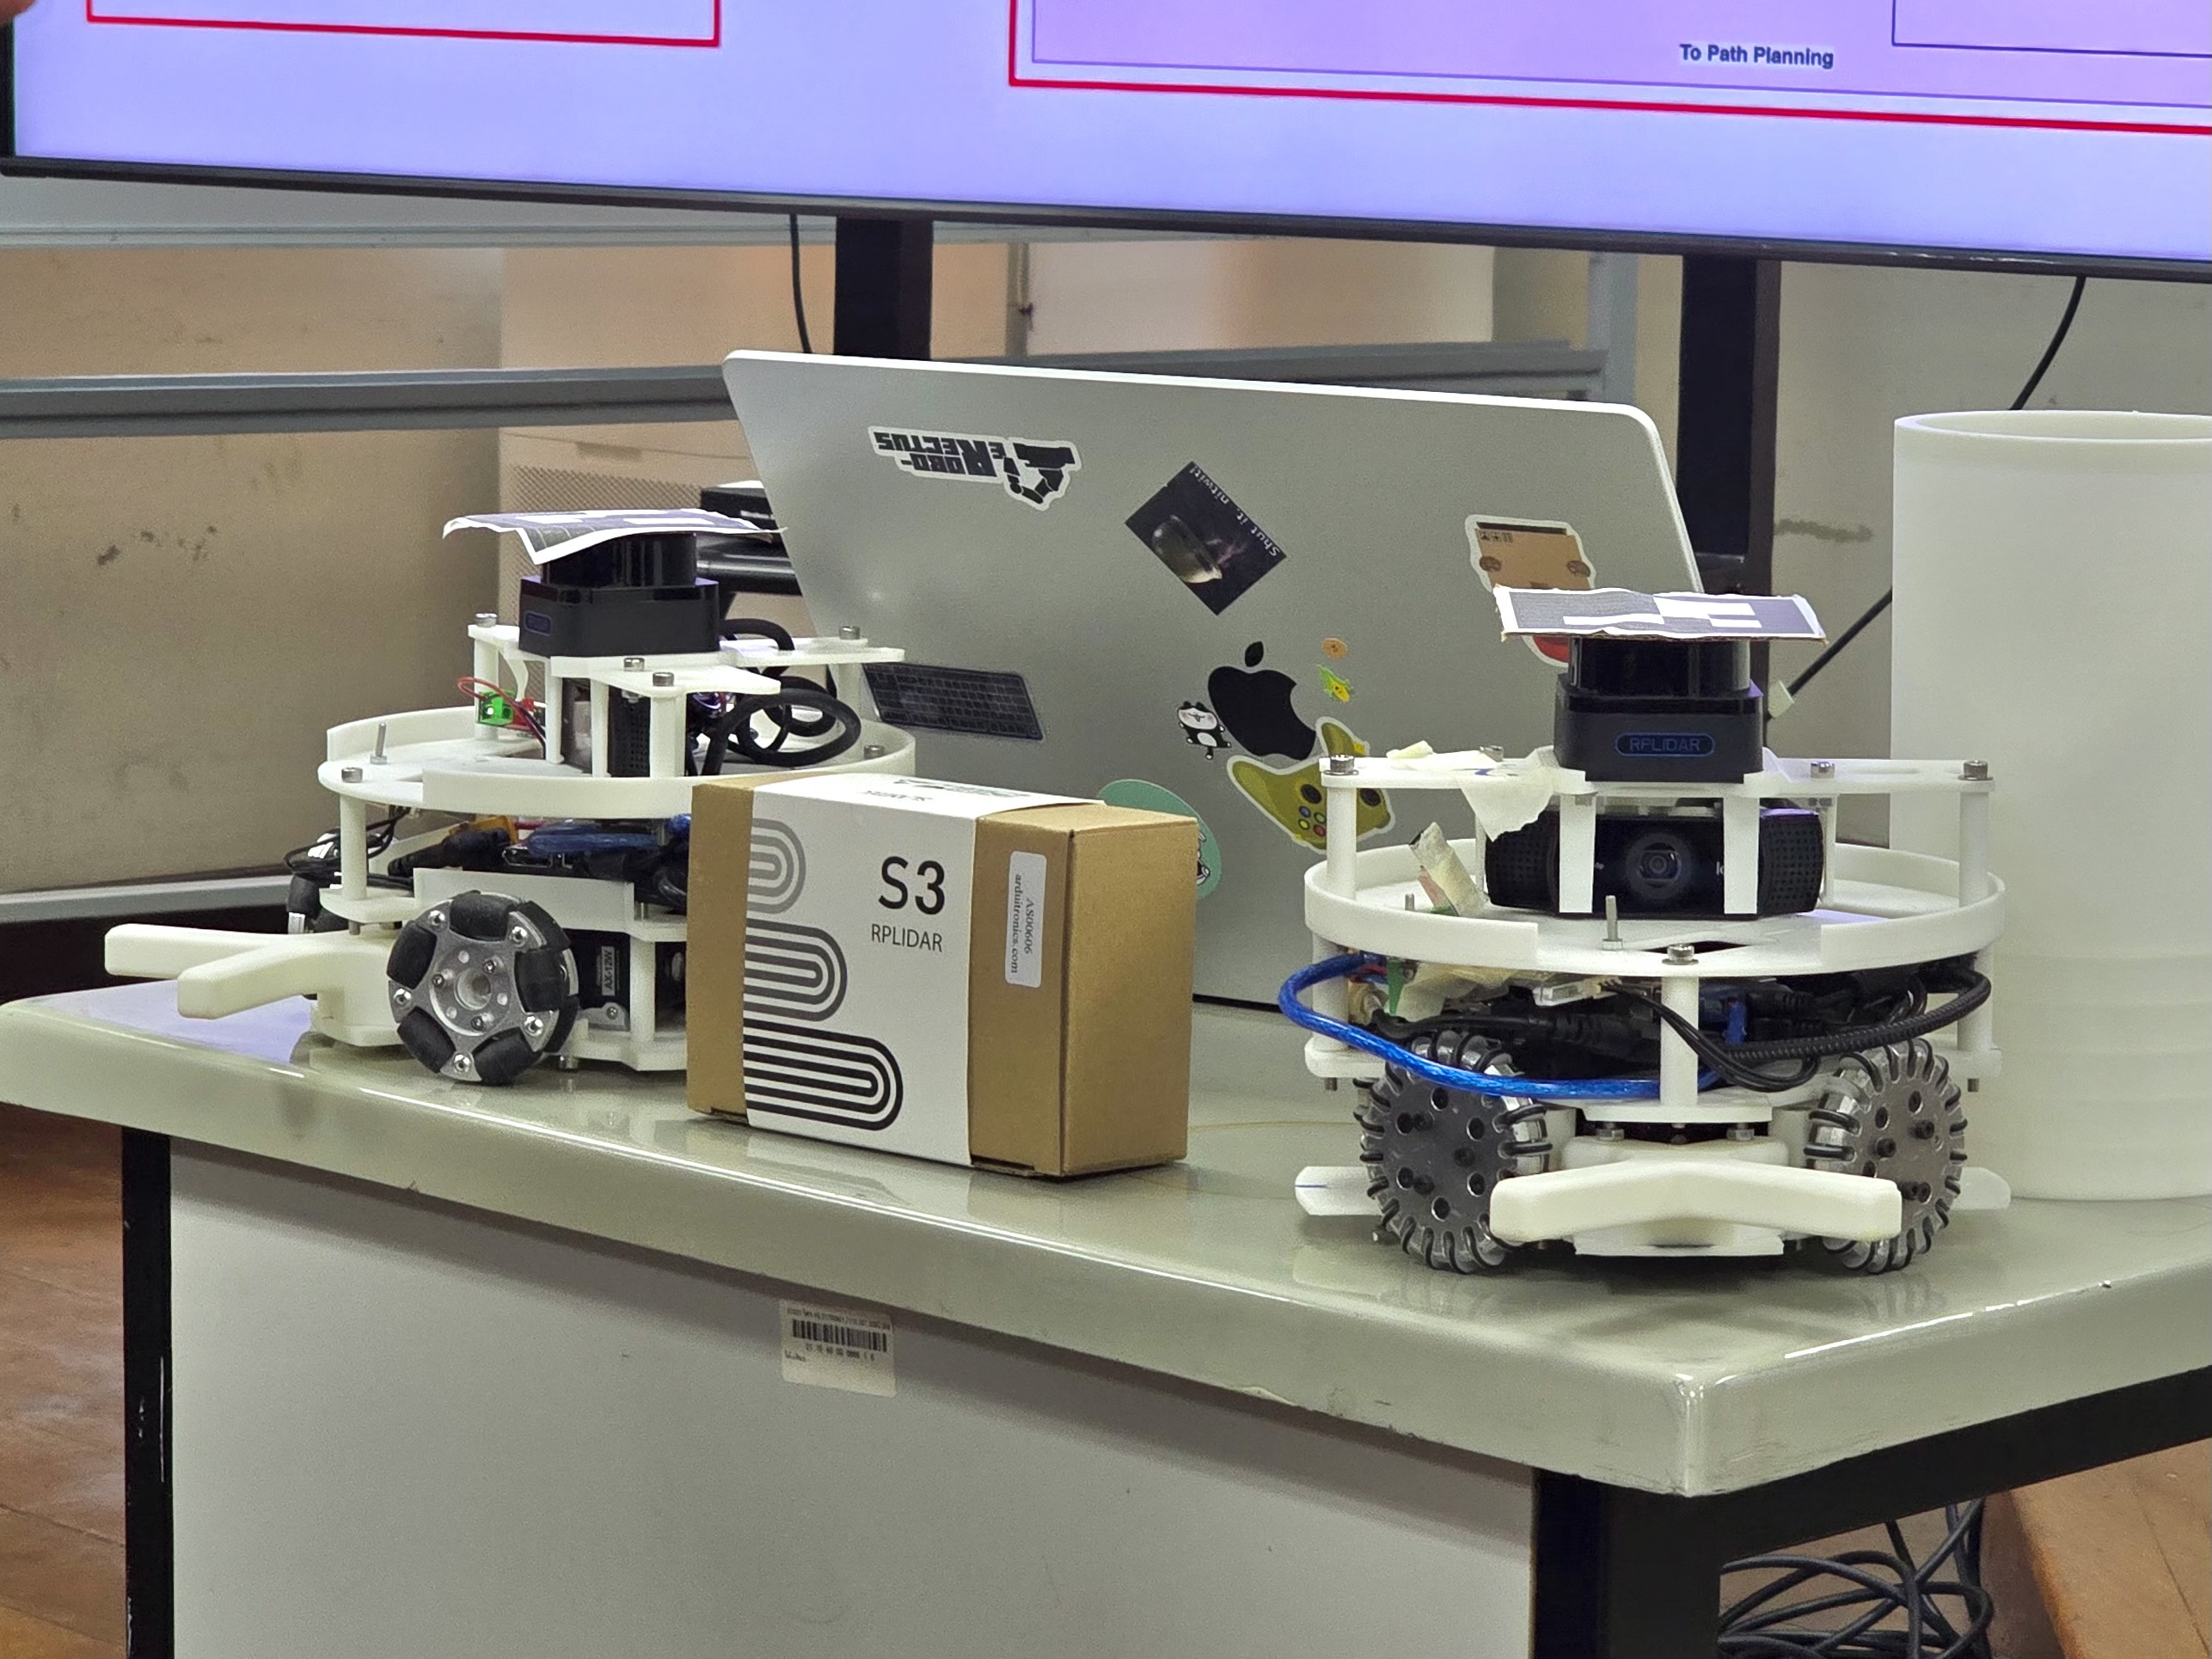
\includegraphics[height=5cm]{assets/images/hardware/irl-2-robots.jpeg}
        \caption{}
        \label{fig:irl-2-robot}
    \end{minipage}
    % \hspace{0.1\textwidth} % Add horizontal space here
    % \begin{minipage}{0.41\textwidth}
    %     % \centering
    %     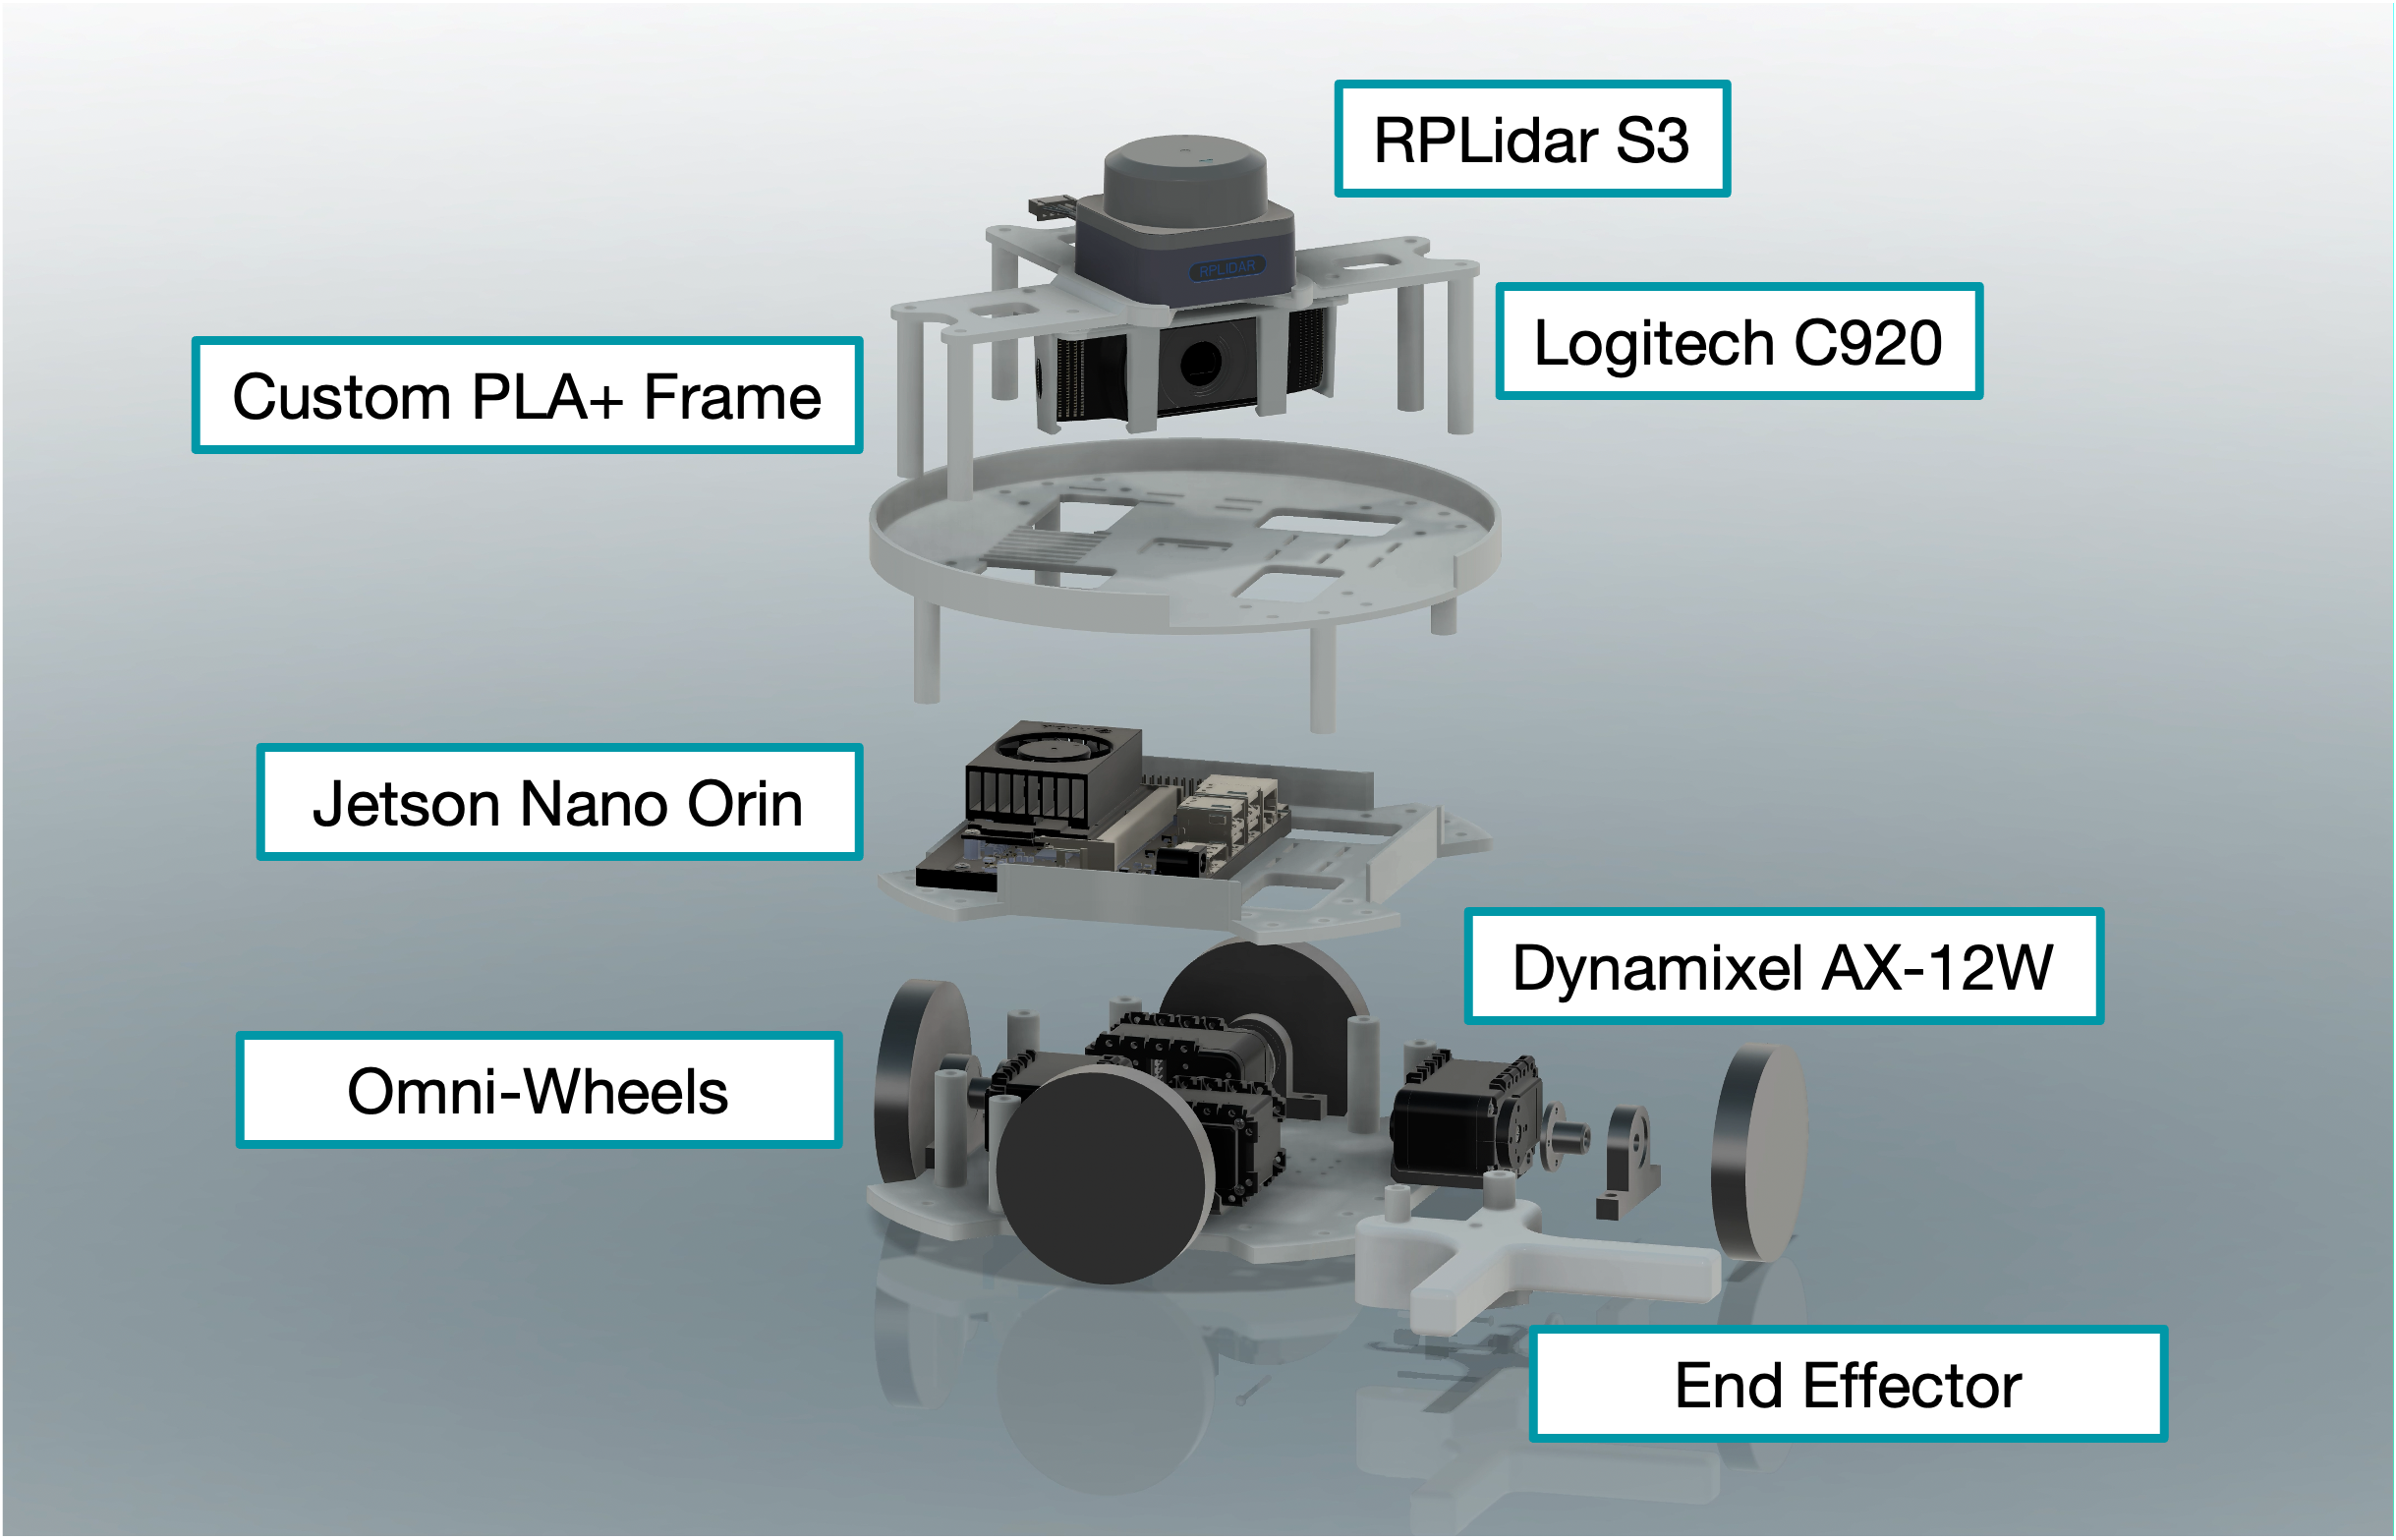
\includegraphics[height=5cm]{assets/images/hardware/robot-exploded-annotated.png}
    %     \caption{CAD Model of Robot Jeff3 annotated}
    %     \label{fig:robot-exploded}
    % \end{minipage}
\end{figure}
% \begin{figure}[!htb]
%     % \centering
%     \begin{minipage}{0.41\textwidth}
%         % \centering
%         \includegraphics[height=5cm]{assets/images/hardware/}
%         \caption{}
%         \label{fig:}
%     \end{minipage}
%     \hspace{0.1\textwidth} % Add horizontal space here
%     \begin{minipage}{0.41\textwidth}
%         % \centering
%         \includegraphics[height=5cm]{assets/images/hardware/}
%         \caption{}
%         \label{fig:}
%     \end{minipage}
% \end{figure}

% \begin{figure} [H]
%     \centering
%     \begin{tabular}{@{}c@{\hspace{0.5cm}}p{8cm}@{\hspace{0.5cm}}c@{}}
%         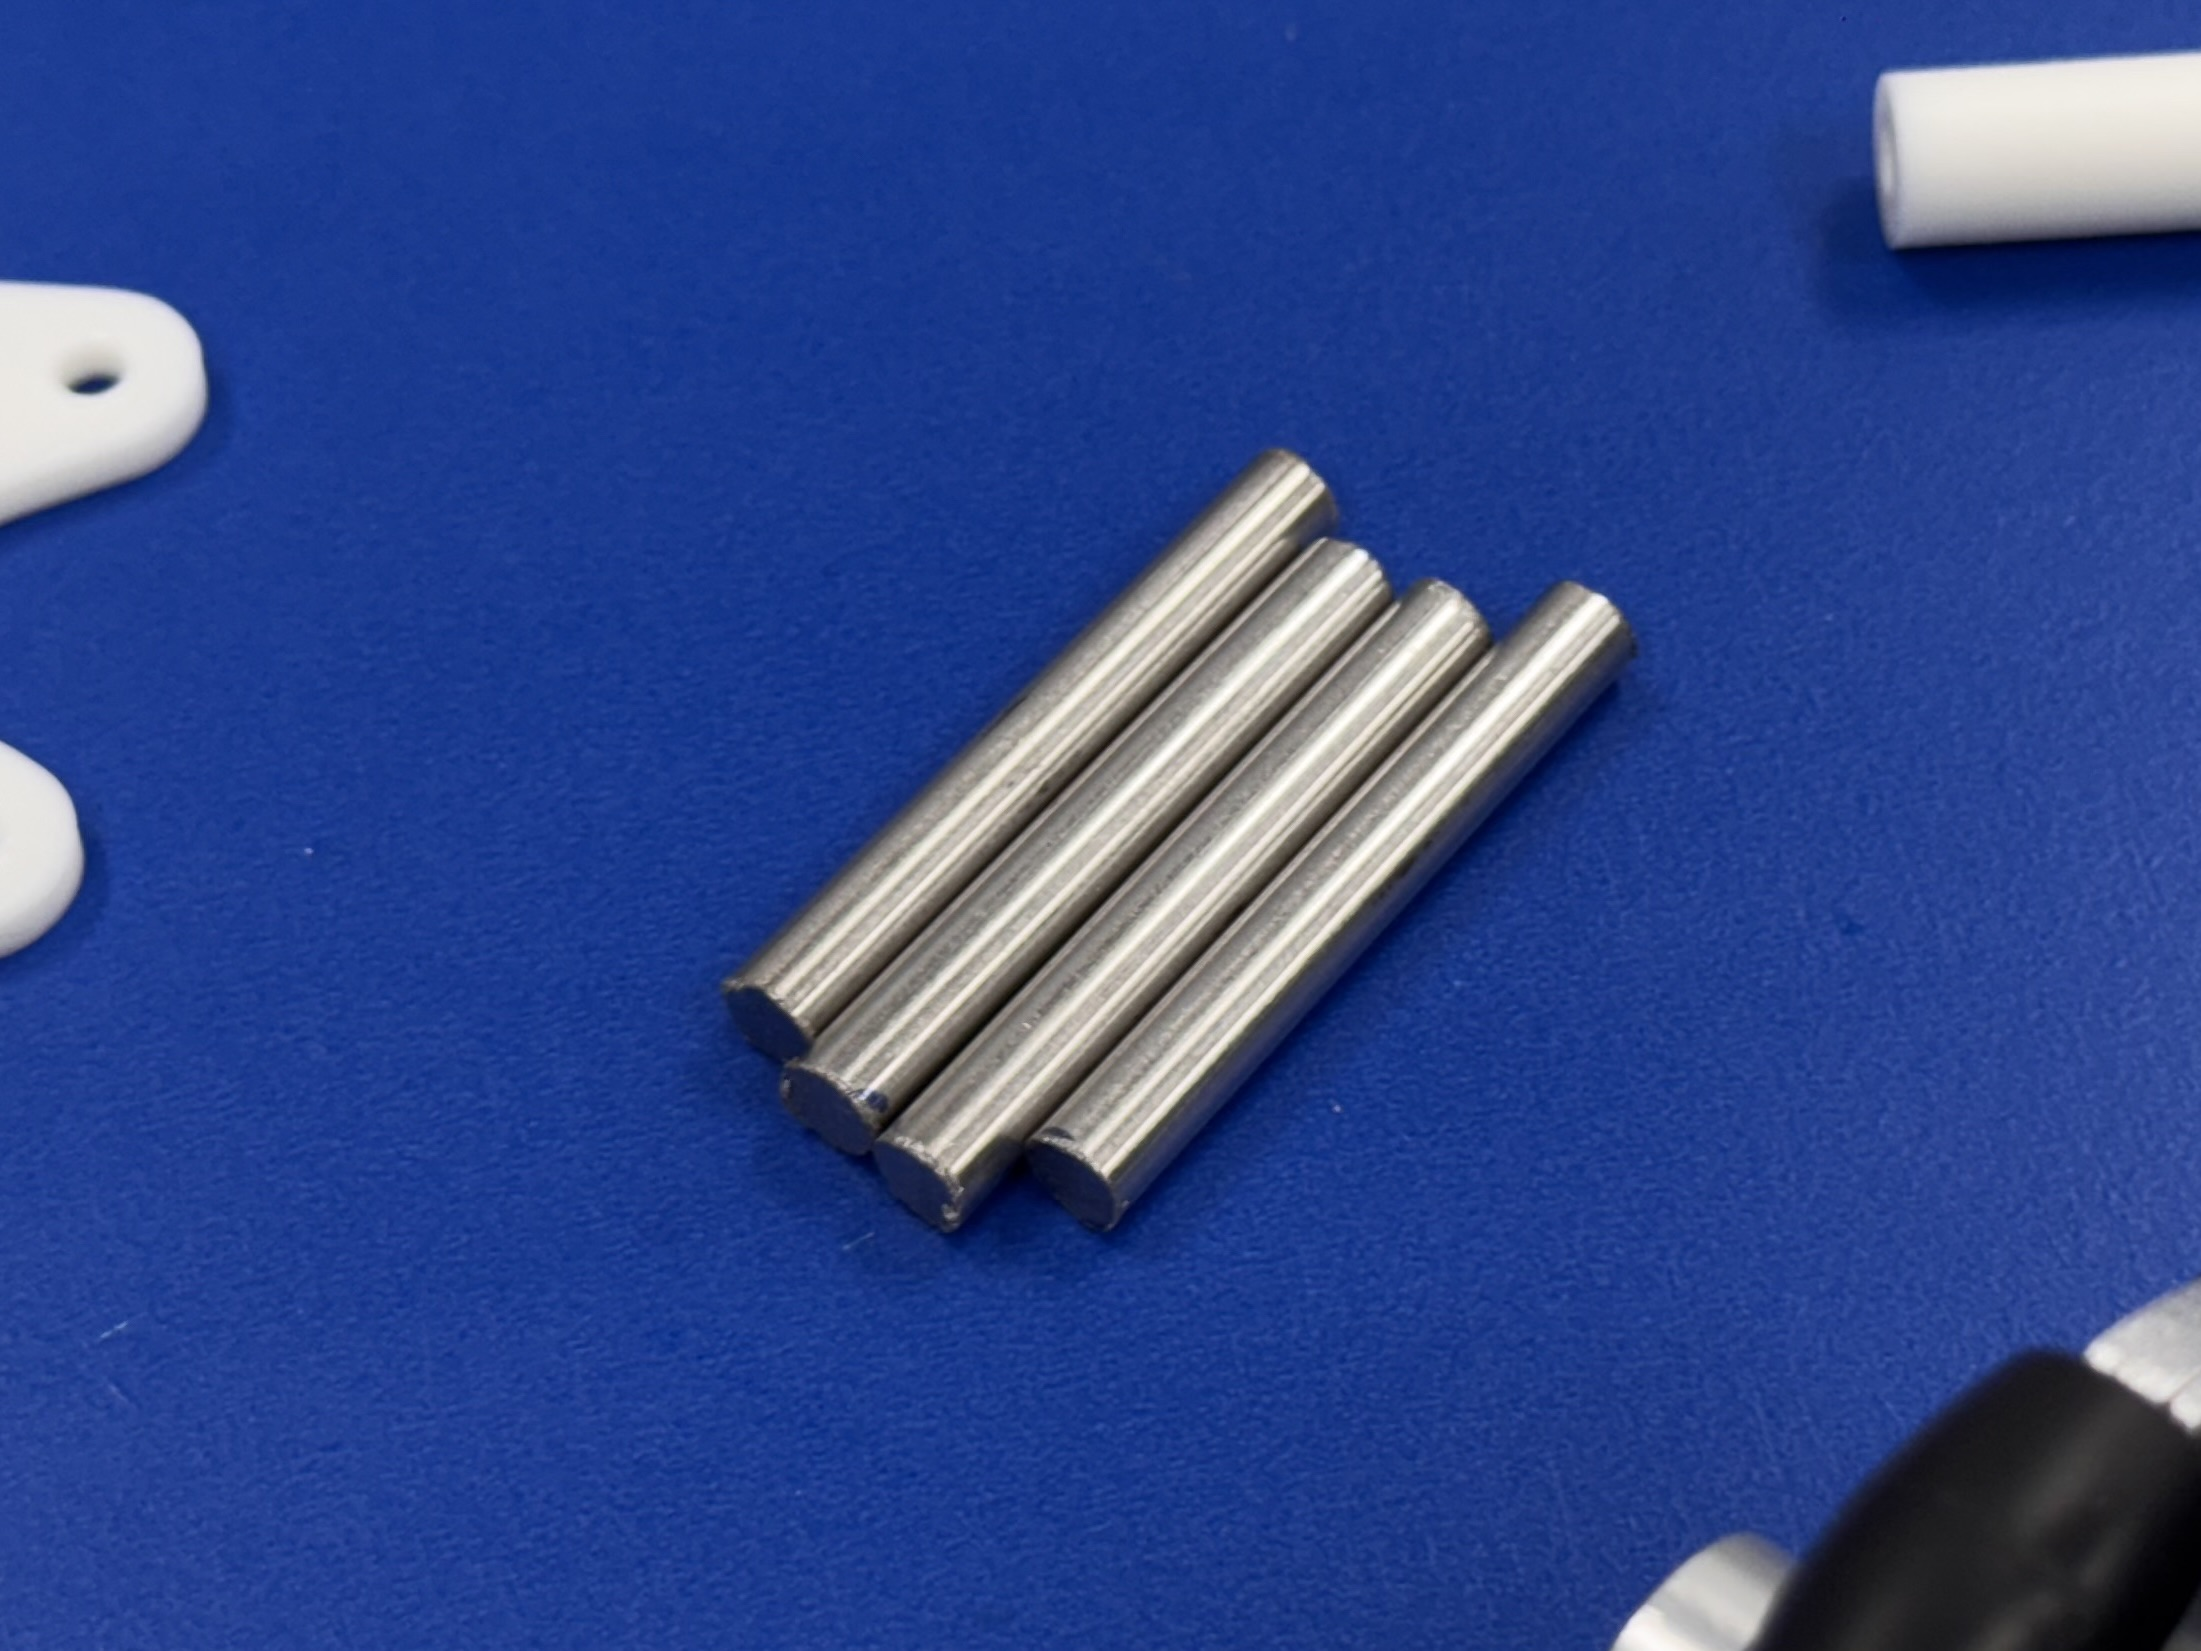
\includegraphics[width=0.5\textwidth]{assets/images/hardware/IMG_8280.jpeg} &
%         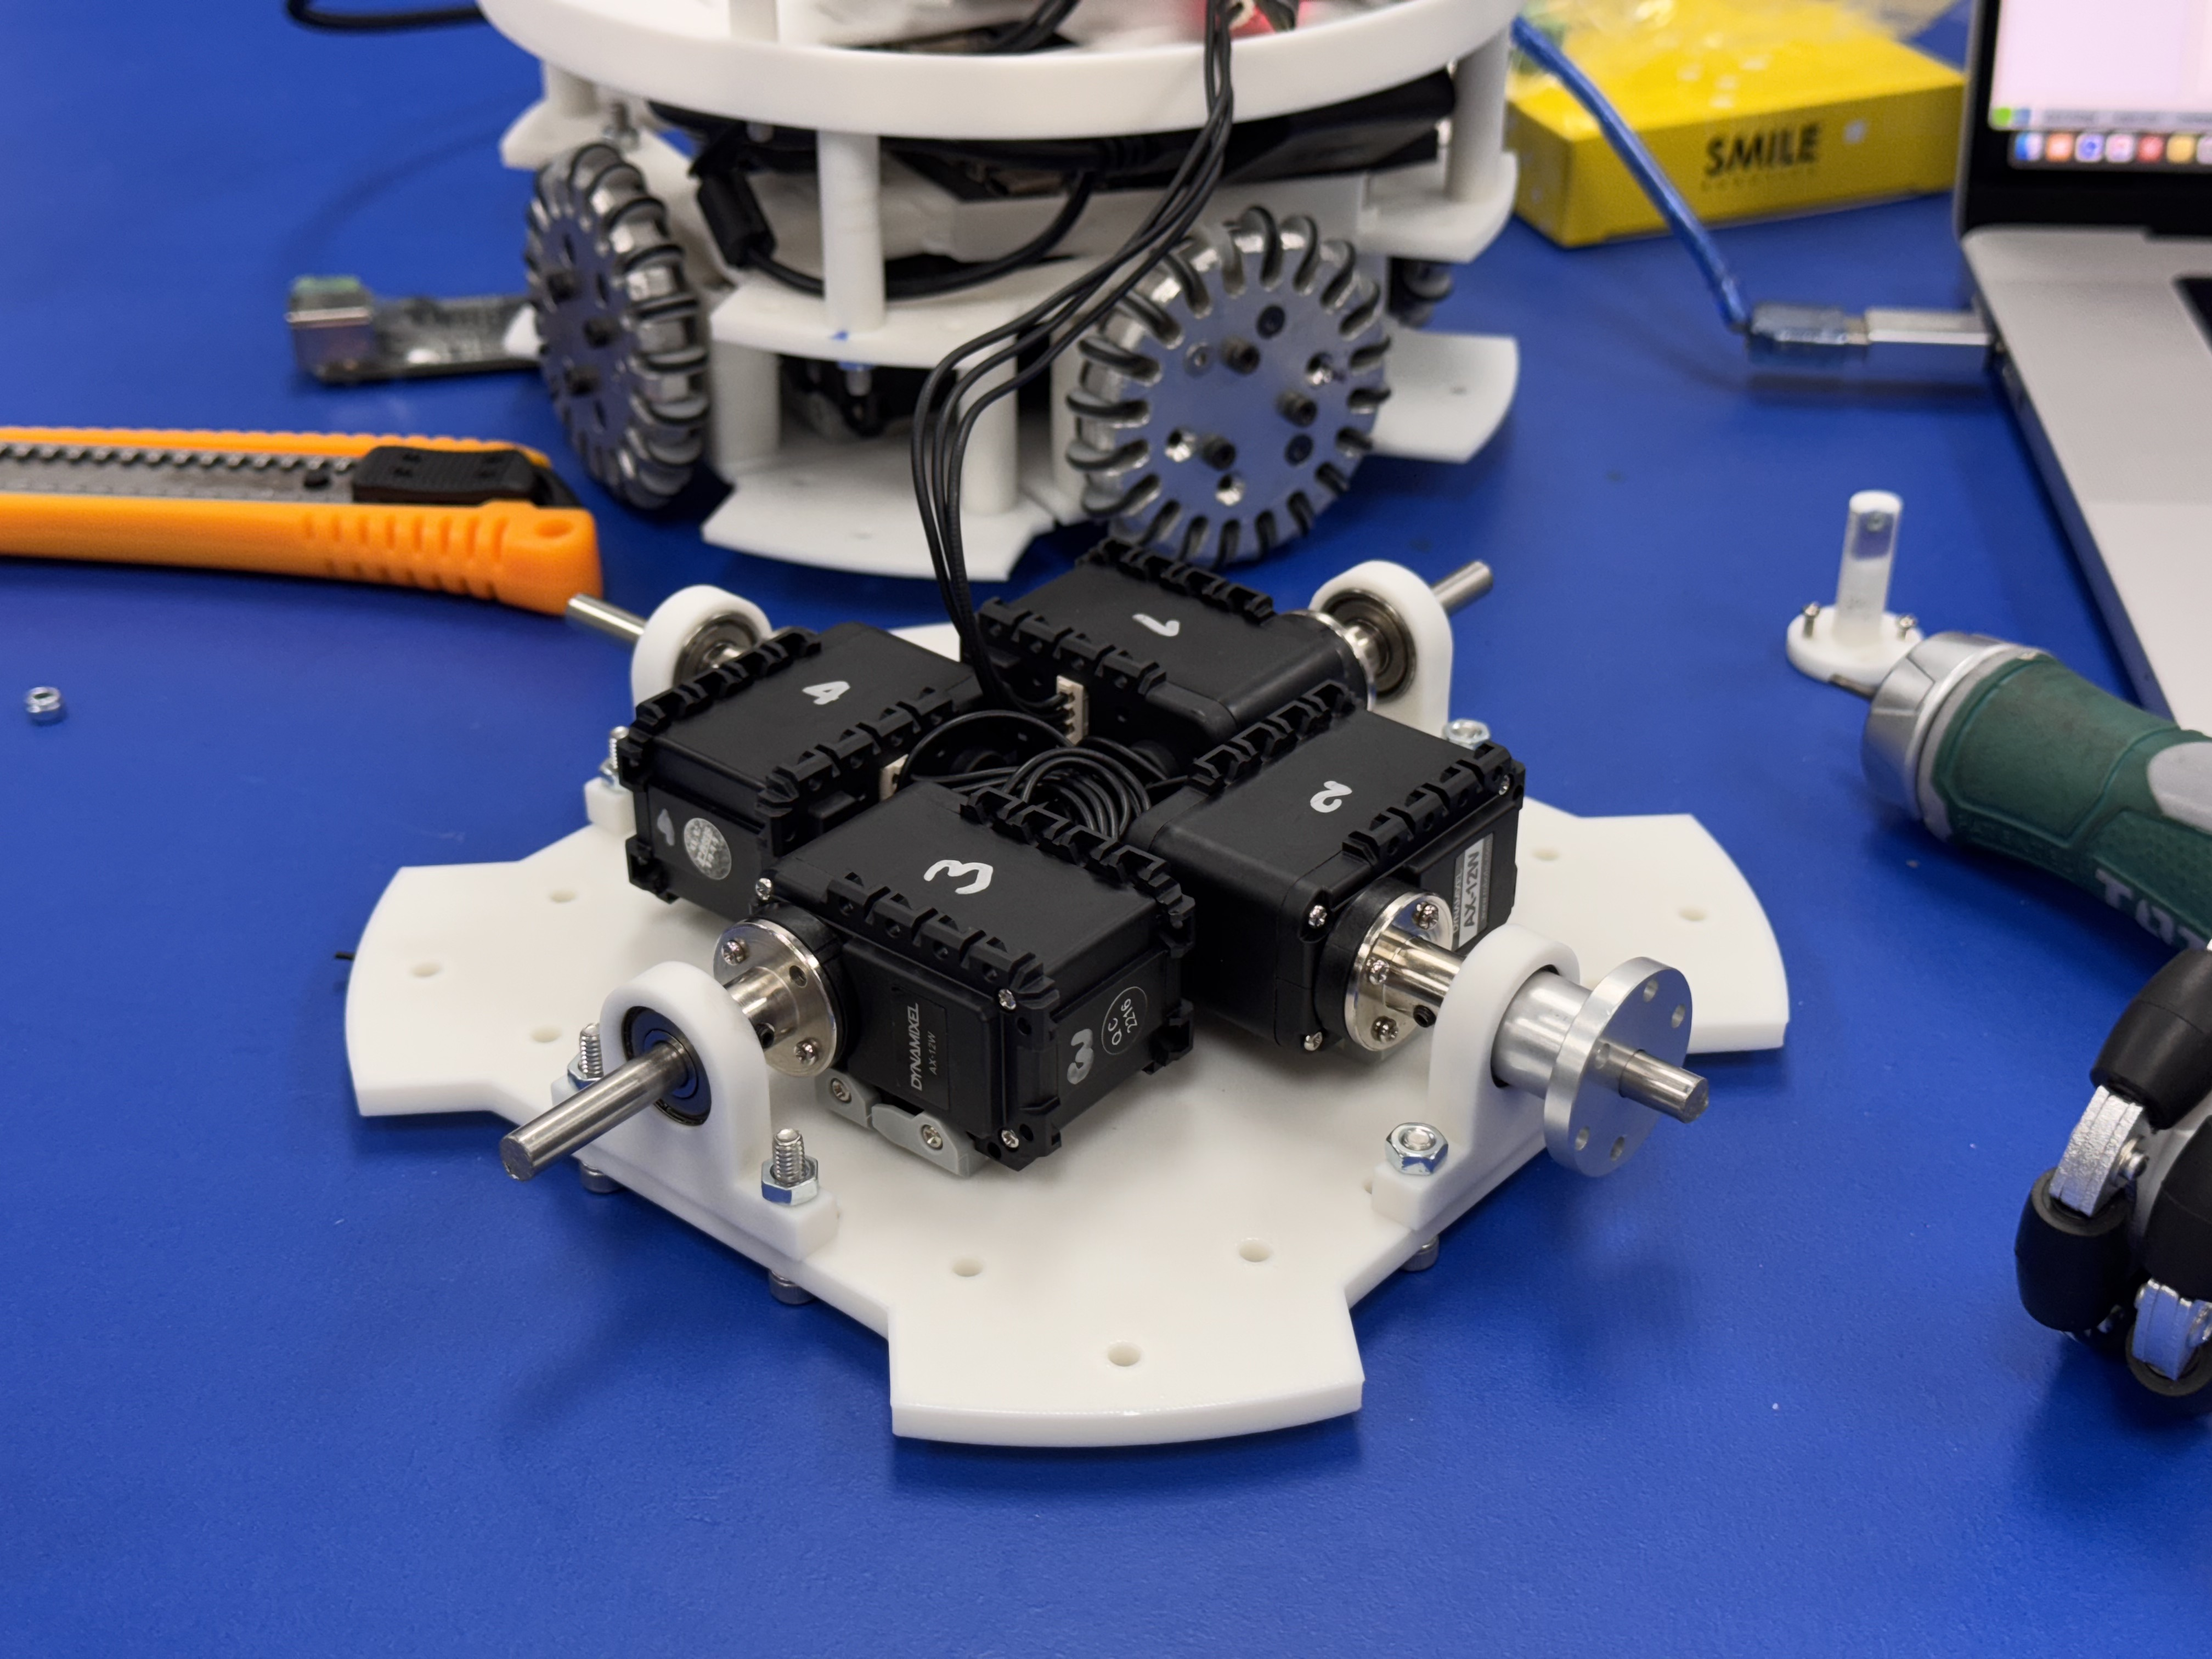
\includegraphics[width=0.5\textwidth]{assets/images/hardware/IMG_8284.jpeg} & \\
%         \small Sliced Metal Shafts &
%         \small Assembly of the motors, motor flange, bearing pillow block, omni-wheel flange&
%     \end{tabular}
%     \caption{}
%     \label{fig:}
% \end{figure}



\begin{figure} [H]
    \centering
    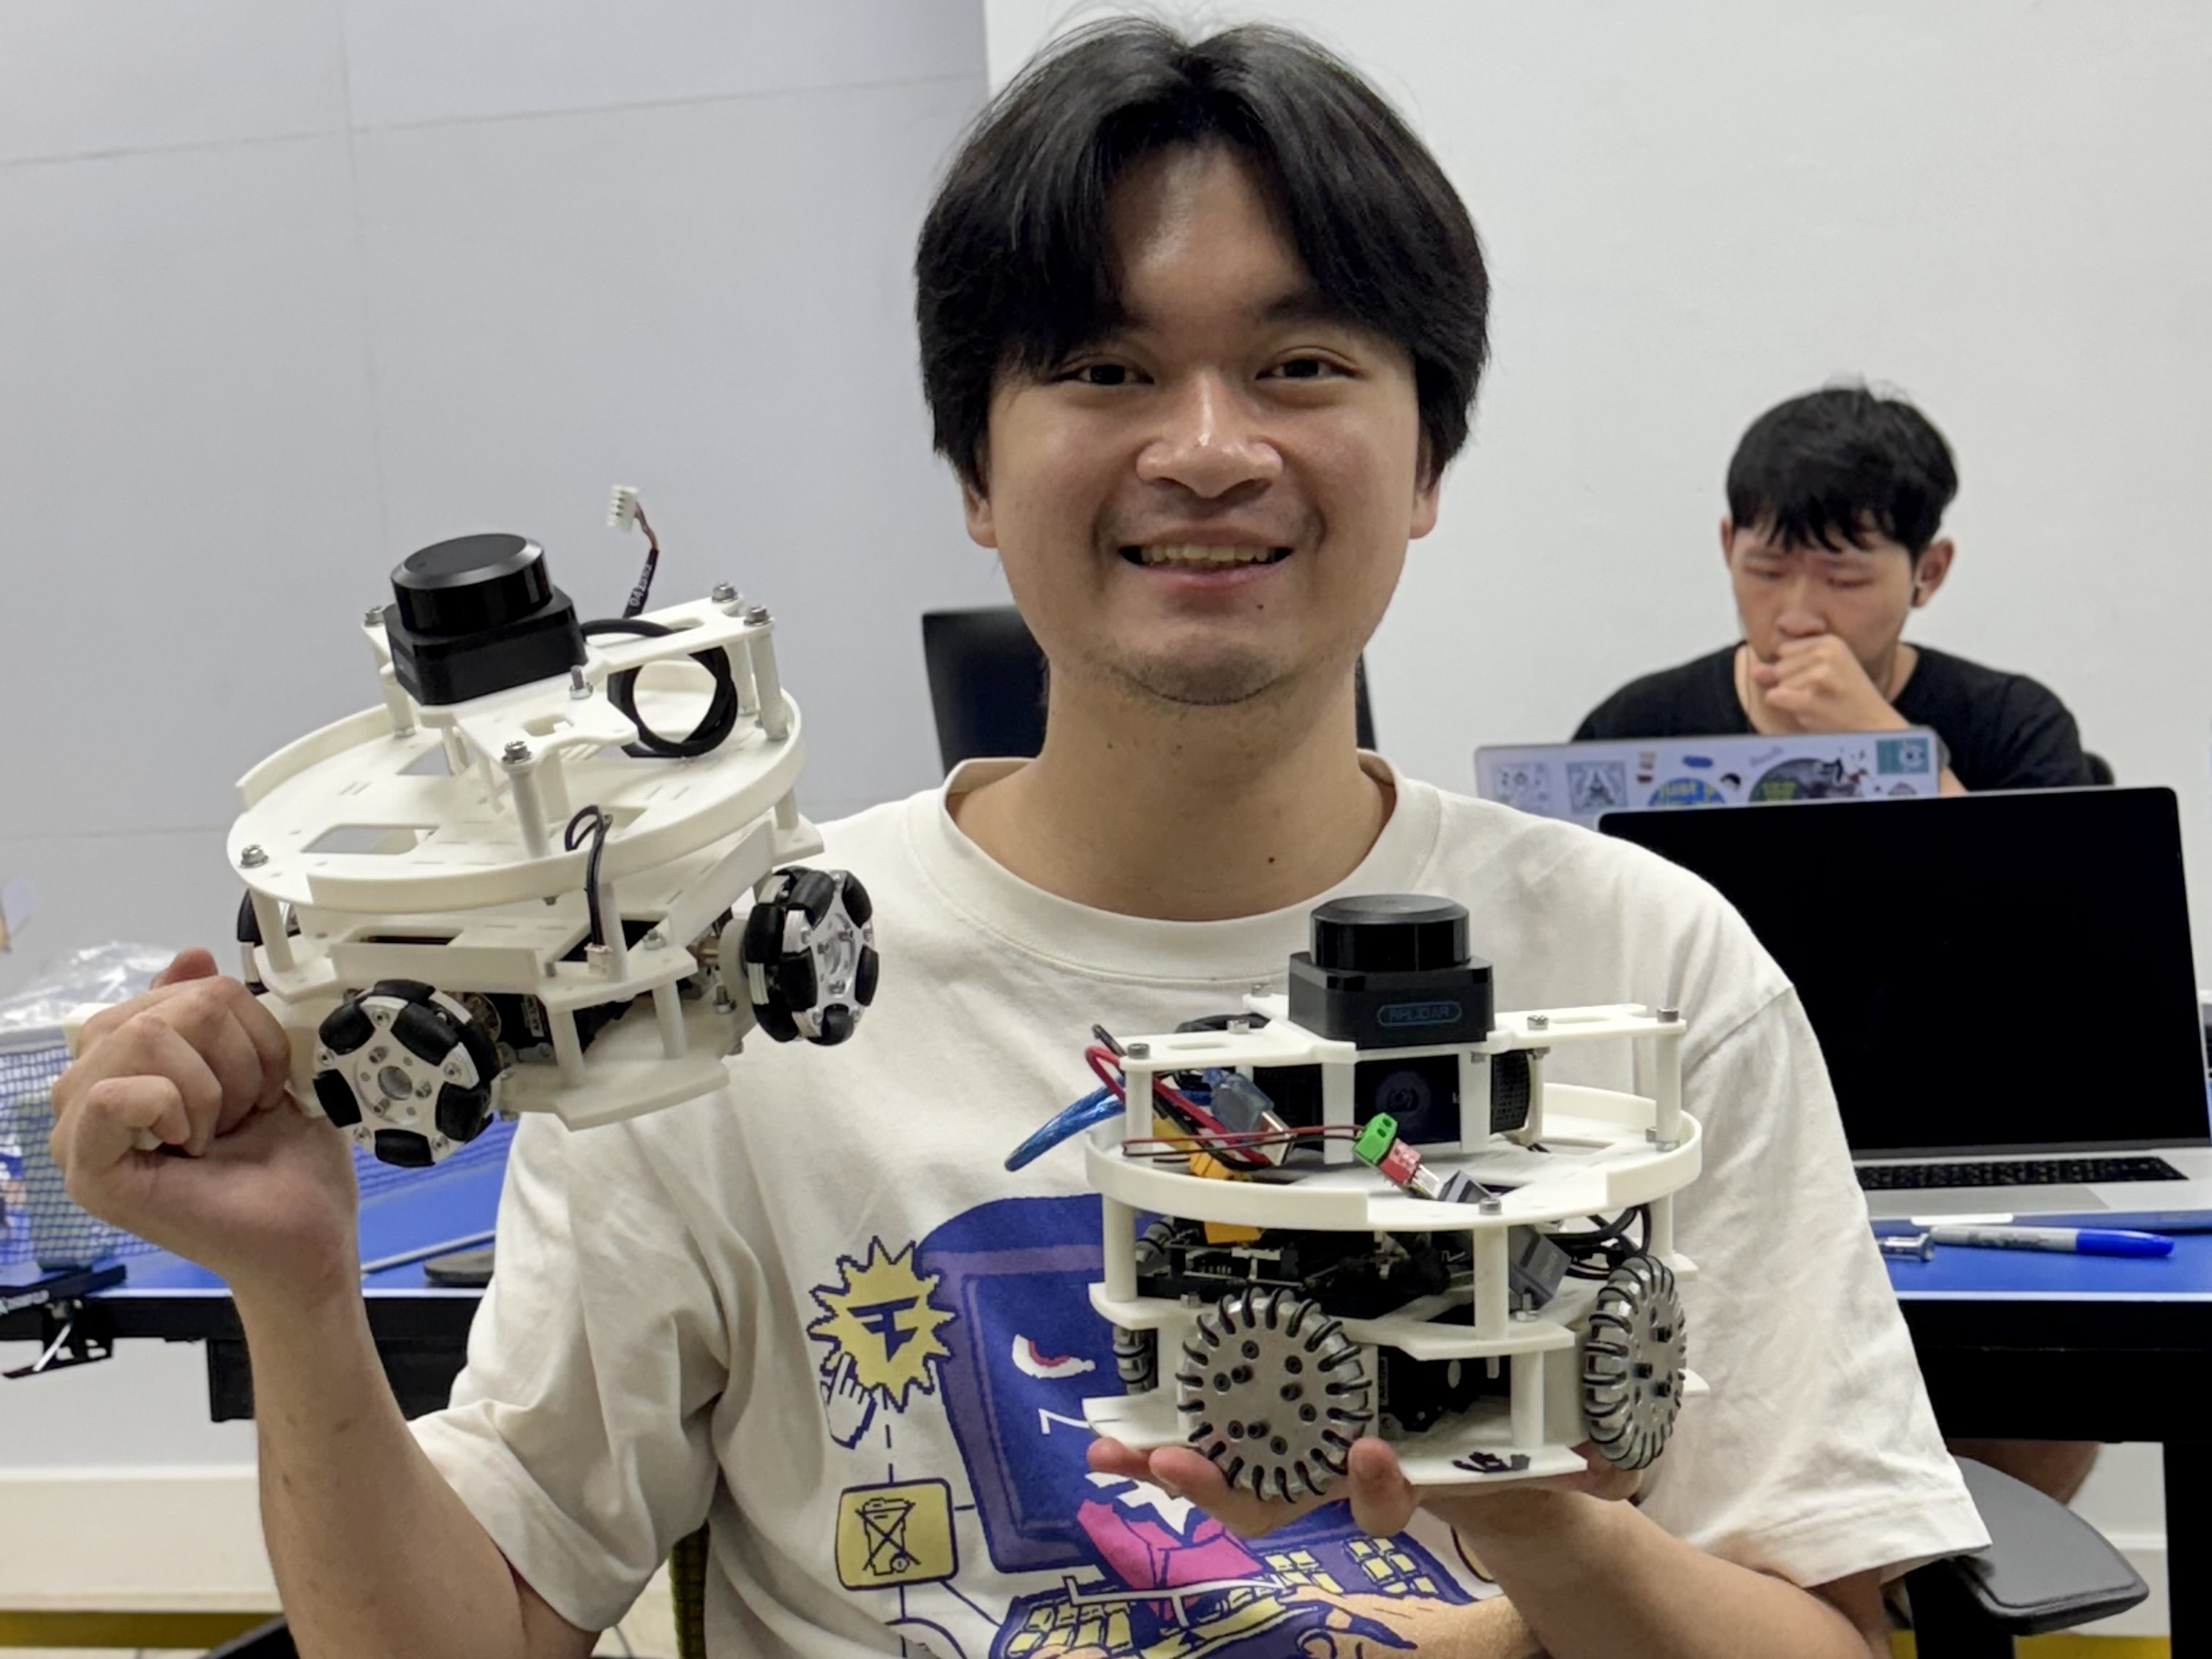
\includegraphics[width=0.65\linewidth]{assets/images/hardware/IMG_8290.jpeg}
    \caption{A happy man holding 2 built robots "Jeff3.0"}
    \label{fig:have2robots}
\end{figure}


Following are the Bill of Material(BOM) cost of one robot: 
\begin{enumerate}
    \item 4x Dynamixel Motors AX-12W - 2,100THB each
    \item 4x Omnidirectional wheels - 980THB each 
    \item 4x Bearing 626ZZ 06x19x06mm - 30THB each
    \item 1x RPLidar S3 Lidar - 23,850THB each 
    \item 1x Logitech C920 RGB Camera - 3,460THB each
    \item 1x Jetson Orin Nano 14,600THB each
    \item 1x USB - TTL board - 400THB each
\end{enumerate}
Total 48,454THB per robot, important to iterate this a proof of concept of a decentralized system, not for commercialization.


% ---------------------------------------------------------------------------------------------------------
\section{Forward and Inverse kinematic of the robot}
\[
\dot{\mathbf{q}} = J^{-1} \cdot \dot{\mathbf{P}}
\]

In this expression, $\dot{q} \in R^4$ is the vector of angular velocities of the four drive wheels, while $\dot{P} \in R^3$ is the platform velocity vector consisting of the forward velocity $V_x$, lateral velocity $V_y$, and yaw rate $\dot{\theta}_z$. The inverse Jacobian matrix $J^{-1}$ relates the platform motion to the required wheel speeds, based on the robot's kinematic configuration.

For the X-drive configuration, the Jacobian takes the following matrix form:

\begin{figure}[H]
\[
\begin{bmatrix}
\dot{q}_1 \\
\dot{q}_2 \\
\dot{q}_3 \\
\dot{q}_4 \\
\end{bmatrix}
=
\frac{1}{r}
\begin{bmatrix}
-\sin(\theta + \frac{\pi}{4}) & \cos(\theta + \frac{\pi}{4}) & R \\
-\sin(\theta + \frac{3\pi}{4}) & \cos(\theta + \frac{3\pi}{4}) & R \\
-\sin(\theta + \frac{5\pi}{4}) & \cos(\theta + \frac{5\pi}{4}) & R \\
-\sin(\theta + \frac{7\pi}{4}) & \cos(\theta + \frac{7\pi}{4}) & R \\
\end{bmatrix}
\begin{bmatrix}
V_x \\ 
V_y \\
\dot{\theta}_z \\
\end{bmatrix}
\]
\caption{Wheel velocity calculation using the inverse Jacobian matrix. The vector on the left-hand side \( [\dot{q}_1, \dot{q}_2, \dot{q}_3, \dot{q}_4]^T \) represents the angular velocities of the four wheels. The Jacobian matrix reflects the X-drive wheel configuration. In this context, \( \theta \) is the robot's global orientation, \( R \) is the radial distance from the robot's centre to each wheel, and \( r \) is the wheel radius. The input vector on the right-hand side comprises \( V_x \) and \( V_y \), the body-frame linear velocities, and \( \dot{\theta}_z \), the angular velocity about the vertical axis.}
\label{fig:matrix-wheel}
\end{figure}

Each resulting wheel angular velocity \( \dot{q}_i \) is then used as a target input to a local PID controller, which ensures the wheel reaches and maintains this desired velocity. The control law is based on the difference between the target and measured angular velocities of the wheel:

\[
e_i(t) = \dot{q}_i^{\text{target}}(t) - \dot{q}_i^{\text{measured}}(t)
\]

The control input \( u_i(t) \), which is applied to the motor driver, is then computed using the standard PID formulation:

\[
u_i(t) = K_p e_i(t) + K_i \int_{0}^{t} e_i(\tau)\, d\tau + K_d \frac{d}{dt} e_i(t)
\]

Here, \( e_i(t) \) represents the instantaneous control error at time \( t \), \( K_p \) is the proportional gain that reacts to present error, \( K_i \) is the integral gain that accumulates past error to eliminate steady-state offset, and \( K_d \) is the derivative gain that anticipates future error trends. The PID controller thus dynamically adjusts the motor actuation to match the target wheel velocity, enabling precise and stable tracking of the robot's motion commands.
% ---------------------------------------------------------------------------------------------------------
\section{Base Platform Modification and Microcontroller Integration}
The initial version of the robot was built using Dynamixel AX-12W motors. However, we encountered major issues in odometry due to the low quality and unreliability of the built-in encoders. These limitations hindered accurate velocity and position estimation.

To overcome these issues, we redesigned the robot base. The new design incorporates DC motors equipped with optical encoders mounted on the rear shaft. This design offers improved resolution and provides reliable velocity feedback, which is crucial for accurate closed-loop control.

Figure~\ref{fig:encoder-mounting} shows the configuration, where four DC motors operate in coordination. Each motor is driven by an L298N H-bridge motor driver. The control signals for each driver are generated by an ESP32 microcontroller.

\begin{figure}[H]
    \centering
    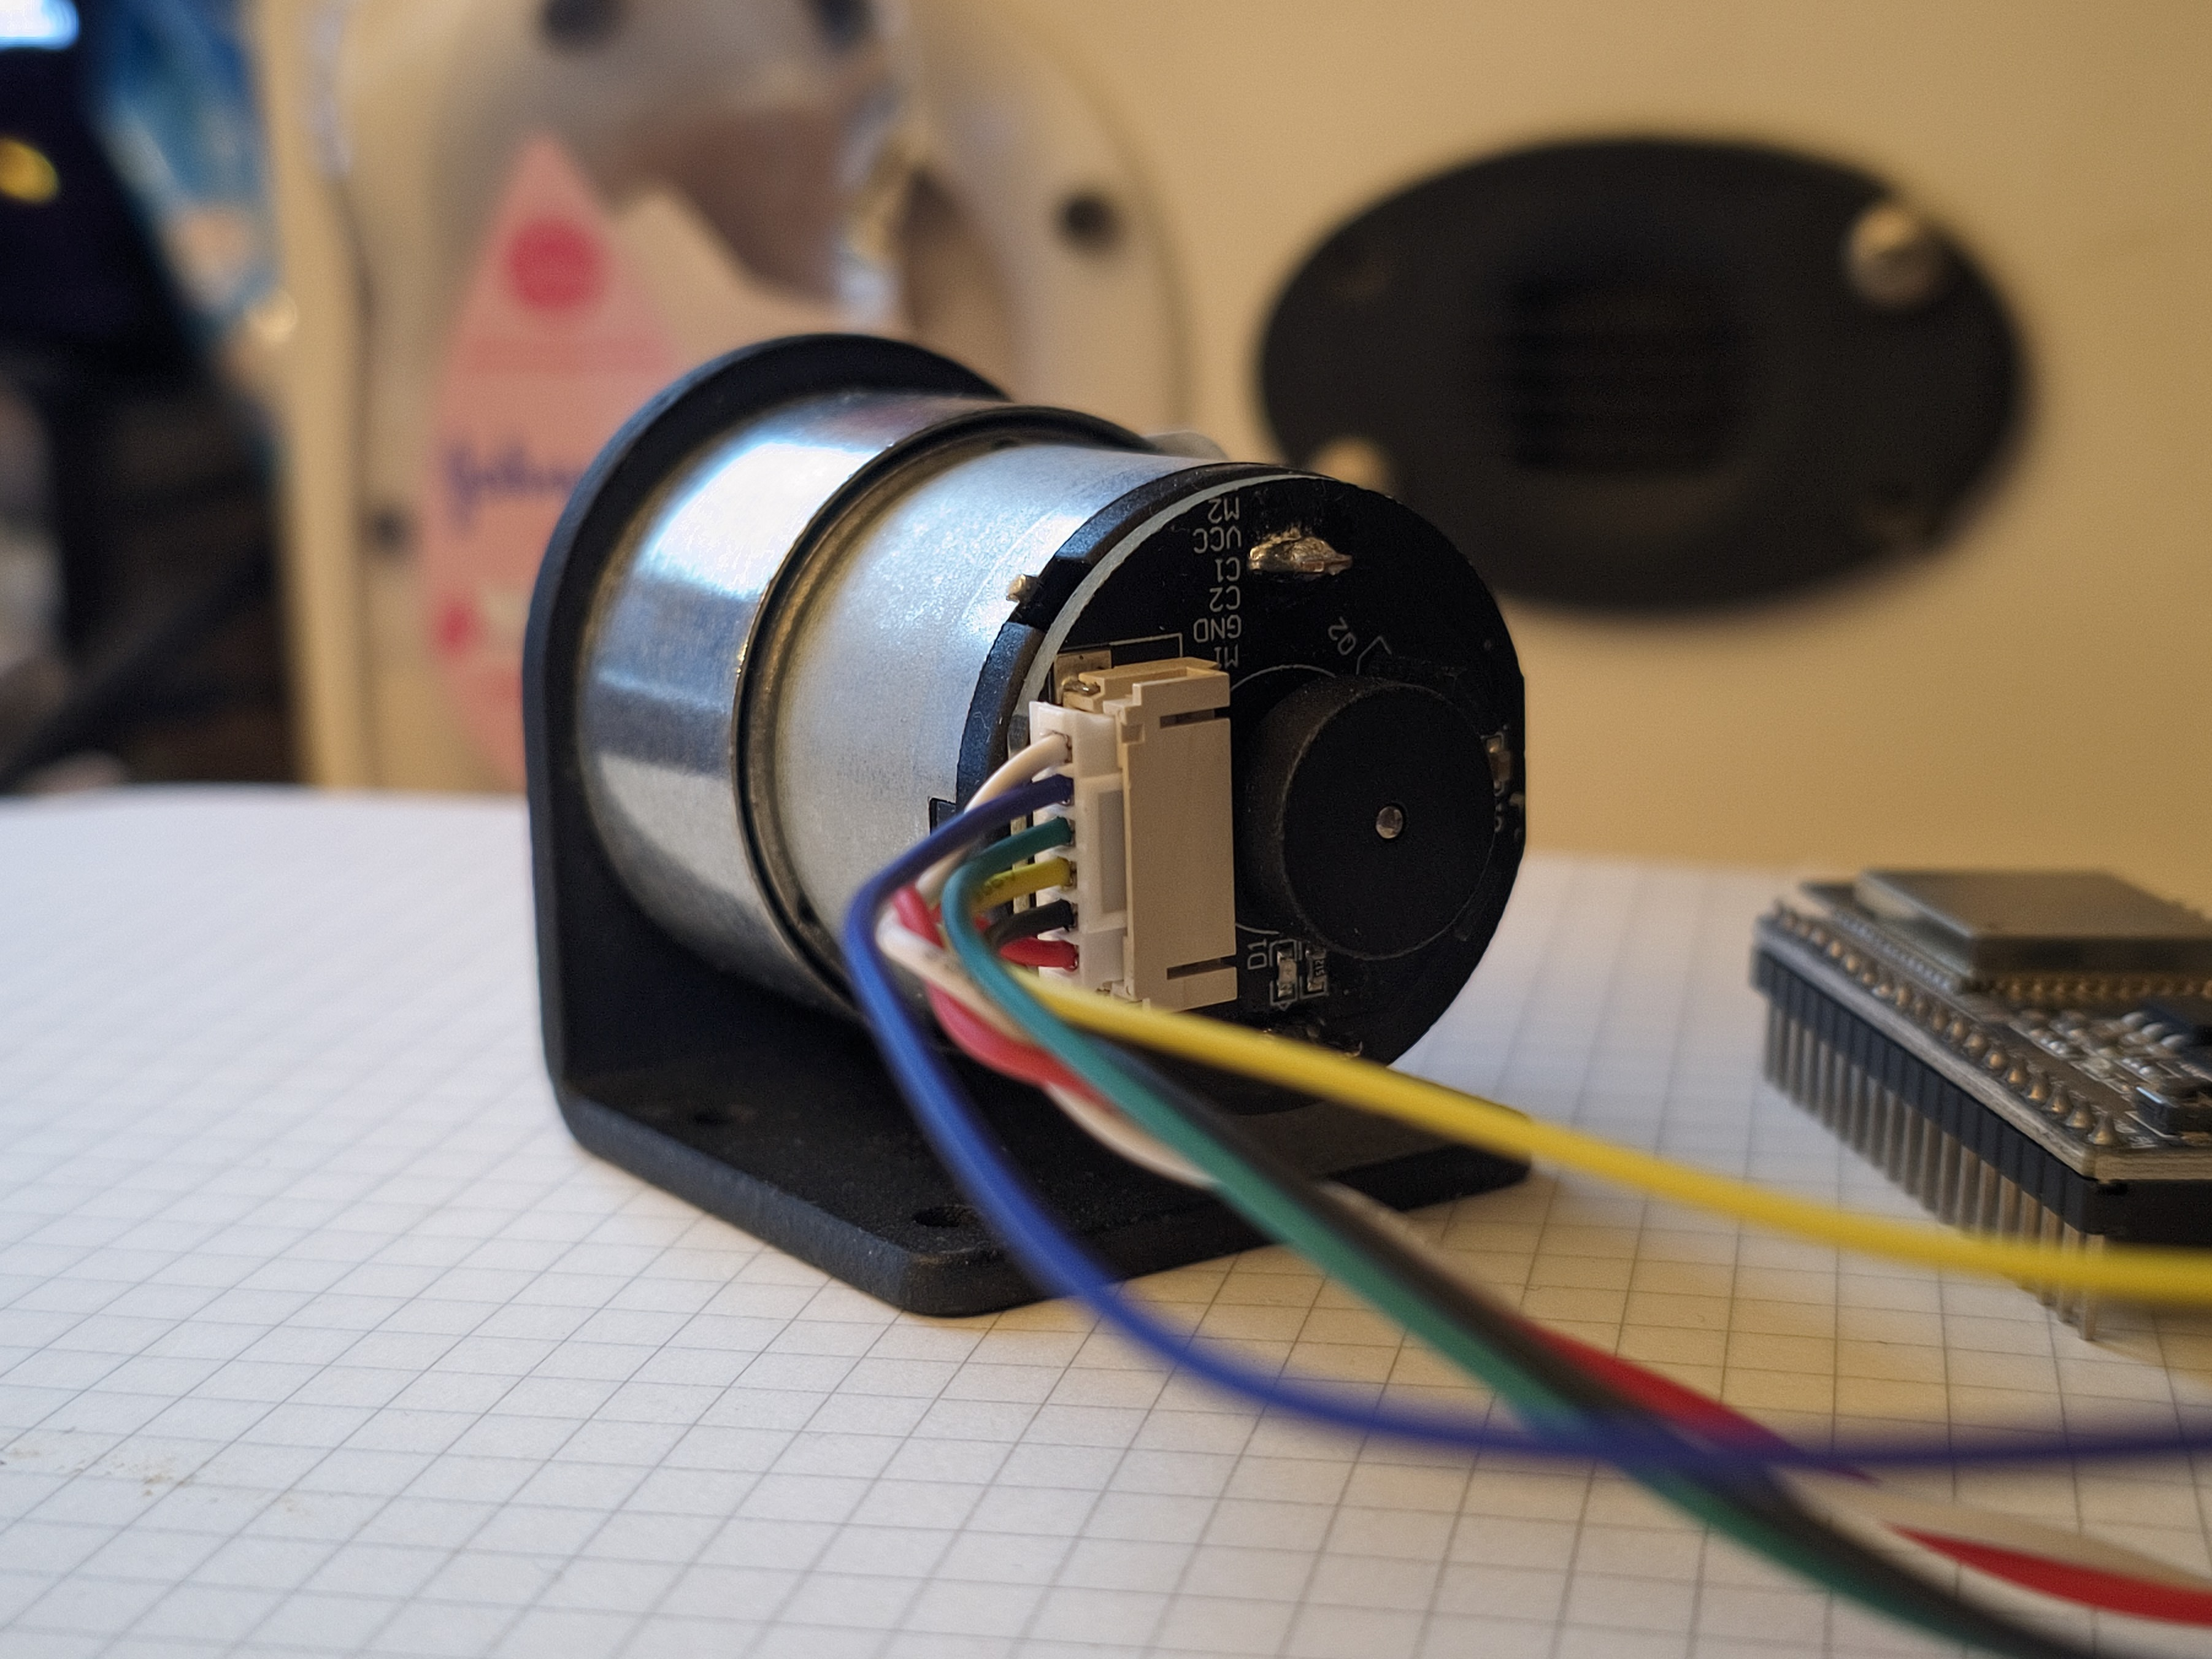
\includegraphics[width=0.6\textwidth]{assets/images/hardware/dc-motor2.jpeg}
    \caption{DC motor with integrated encoder at the rear shaft, enabling closed-loop control.}
    \label{fig:encoder-mounting}
\end{figure}

The ESP32 is programmed using the ESP-IDF framework, which is based on FreeRTOS. Unlike the Arduino framework, ESP-IDF provides direct access to low-level resources and supports real-time scheduling. This choice removes the overhead introduced by Arduino’s abstraction layers and enables finer control over timing and concurrency. As a result, we achieve more accurate and responsive motor control.

The new platform design and software stack lay the foundation for the following section, which describes the detailed architecture of the motor control system.